\scanpage{1}
\figure{%
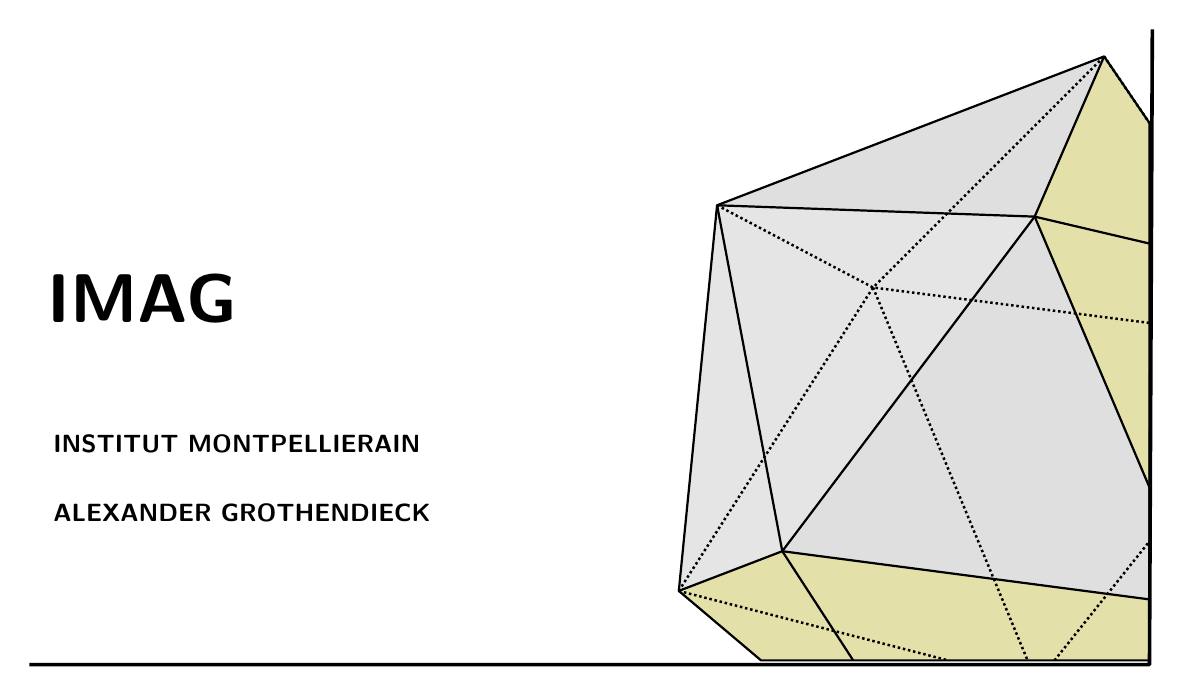
\begin{tikzpicture}[x=0.018cm,y=-0.018cm,line join=round]
\node[anchor=west,font=\sffamily\bfseries\fontsize{64}{64}\selectfont] at (18,203) {IMAG};
\node[anchor=west,font=\sffamily\bfseries\small] at (22,305) {INSTITUT MONTPELLIERAIN};
\node[anchor=west,font=\sffamily\bfseries\small] at (22,354) {ALEXANDER GROTHENDIECK};
\fill[gray!25] (497,137)--(770,32)--(721,145)--cycle;
\fill[gray!20] (497,137)--(721,145)--(543,381)--cycle;
\fill[gray!25] (543,381)--(721,145)--(802,336)--(802,415)--cycle;
\fill[gray!20] (497,137)--(543,381)--(470,409)--cycle;
\fill[olive!25] (770,32)--(802,79)--(802,164)--(721,145)--cycle;
\fill[olive!25] (721,145)--(802,164)--(802,336)--cycle;
\fill[olive!25] (470,409)--(543,381)--(593,458)--(528,458)--cycle;
\fill[olive!25] (543,381)--(802,415)--(802,458)--(593,458)--cycle;
\draw[line width=0.8pt] (497,137)--(770,32)--(802,79)--(802,458)--(528,458)--(470,409)--cycle;
\draw[line width=0.8pt] (497,137)--(721,145)--(802,164);
\draw[line width=0.8pt] (770,32)--(721,145)--(543,381)--(470,409);
\draw[line width=0.8pt] (721,145)--(802,336);
\draw[line width=0.8pt] (497,137)--(543,381)--(593,458);
\draw[line width=0.8pt] (543,381)--(802,415);
\draw[densely dotted,line width=0.9pt] (497,137)--(607,195)--(802,220);
\draw[densely dotted,line width=0.9pt] (470,409)--(607,195)--(770,32);
\draw[densely dotted,line width=0.9pt] (607,195)--(716,458);
\draw[densely dotted,line width=0.9pt] (470,409)--(660,458);
\draw[densely dotted,line width=0.9pt] (735,458)--(802,374);
\draw[densely dotted,line width=0.9pt] (770,32)--(802,79);
\draw[line width=1.3pt] (12,461)--(802,461)--(804,13);
\end{tikzpicture}%
}

\scanpage{2}
Pages 1-67

\margin{1}

\scanpage{3}
\mspage{\unsure{1}}
1. \uline{Résultats de fidélité}

À tout corps $K$, associons son topos étale $B_K$, qui est un topos (pro\inserted{fini})galoisien. Le groupoïde des points de $B_K$ est noté $\Pi_K$, il est \unsure{antiéquivalent} canoniquement à la catégorie des clôtures alg. séparables de $K$. Si $\bar K$ est une telle clôture, son groupe des \inserted{$K$-}automorphismes $\operatorname{Gal}(\bar K/K)$ ou $E_{\bar K/K}$ s'identifie au groupe des \deleted{$K$-}automorphismes du pt \inserted{de $B_K$} associé à $\bar K/K$ (il vaut peut-être mieux de dire : à l'opposé de ce groupe -- \deleted{$\bar K$} la \unsure{variance} des clôtures alg. de $K$ est comme celle des foncteurs fibres, à l'opposé de celle des points...)

Bien entendu, $B_K$ se reconstitue à partir de $\Pi_K$, comme le topos des systèmes locaux (continus) sur $\Pi_K$ -- et en termes de $E_{\bar K/K}$, comme le topos des Ensembles discrets à action continue de $E_{\bar K/K}$.

Pour un hom de corps $K\longrightarrow K'$,
\margin{2}

\scanpage{4}
i.e. un hom de schémas $\operatorname{Spec}K' - \operatorname{Spec}K$, on a un morphisme de Topos correspondant
\[
(1)\qquad B_{K'}\unsure{-|\longrightarrow}B_{K^{\deleted{\unsure{\prime}}}}
\]
associé à un hom de groupoïdes fond.
\[
(2)\qquad \Pi_{K'}\unsure{\longrightarrow|-}\Pi_{K^{\deleted{\unsure{\prime}}}}.
\]
Ceci s'explicite en disant qu'un \deleted{clôture} objet de $\Pi_{K'}$ (i.e. pt. de $B_{K'}$, ou \unsure{rev.} universel de $B_{K'}$, \deleted{)} ou clôture \deleted{sép.}\inserted{$\bar K'$} de $K'$) en définit un de $\Pi_{K^{\deleted{\unsure{\prime}}}}$ (associé, en prenant $\bar K^{\deleted{\unsure{\prime}}}=$ clôture \inserted{alg.}\deleted{sép} de $K$ dans $\bar K'$) et pour deux pts correspondants, on a un hom des groupes fondamentaux correspondants, qui s'interprète p.ex. comme
\[
(3)\qquad E_{\bar K'/K'}\unsure{-|\longrightarrow}E_{\bar K^{\deleted{\unsure{\prime}}}/K^{\deleted{\unsure{\prime}}}}
\]
et qui permet de reconstituer l'hom. de topos comme une ``restriction des scalaires''.

\margin{\unsure{1}}
L'image de (3) est le sous-groupe fermé de $E_{\bar K/K}$ qui correspond à la sous-extension
\margin{3}

\scanpage{5}
\mspage{2}
\margin{\diagram{\begin{tikzcd}[ampersand replacement=\&,column sep=small,row sep=small]
K\arrow[r,dash]\arrow[dr,dash]\&K'\arrow[dr,dash]\&{}\\
{}\&\bar K\arrow[r,dash]\&\bar K'
\end{tikzcd}}}
$K_1$ de $\bar K/K$, clôture \inserted{alg.} sép. de $K$ dans $K'$, i.e. $K_1=\bar K\cap K'$.

Quand $K'$ est une extension de type fini de $K$, $K_1$ est une ext. finie de $K$, donc on conclut que l'image de (3) est \unsure{tjs} un sous-groupe d'indice fini, égale à $E_{\bar K/K}$ ssi \inserted{$K_1=K$ i.e.} $K$ est séparablement alg. clos dans $K'$. D'ailleurs, on montre sans mal que \inserted{(si $K'$ est ext. de type fini)} l'hom (3) est injectif ssi $K'$ est une extension algébrique de $K$. Donc il est bijectif ssi $K'$ est une extension radicielle de $K$. Dans la suite nous nous bornerons (provisoirement) aux corps de car. $0$, et la condition précédente \uline{signifie} \inserted{donc} que $K\unsure{-|\longrightarrow}K'$ est un \uline{isomorphisme}.

Ainsi, le foncteur $K\longrightarrow B_K$ ou $K\unsure{-|\longrightarrow}\Pi_K$, ou $(K,\bar K)\unsure{-|\longrightarrow}E_{\bar K/K}$, est \uline{conservatif} quand on se limite comme morphismes de corps \inserted{$K\longrightarrow K'$ (de car. $0$)} à ceux \deleted{pour} qui font de $K'$ une ext. de type fini de $K$.
\margin{4}

\scanpage{6}
P.ex. il suffit de se limiter aux extensions de type fini du corps premier $Q$ -- on trouve un foncteur conservatif de la cat. de ces corps dans celle des groupoïdes \inserted{(ou des topos)}, au sens : un morphisme de corps qui donne une équivalence de groupoïdes (ou de Topos) est un \uline{iso}.

\margin{en car $\unsure{p>0|p\ne0}$ le foncteur est conservatif si de plus on passe à la catégorie \unsure{quot$^t$|quotient} de celle des corps où une extension radicielle finie est considérée comme triviale... (le foncteur $K\unsure{-|\longrightarrow}B_K$ ou $K\unsure{-|\longrightarrow}\Pi_K$ se factorise par cette cat. quotient.)}

Quand on prend des corps quelconques, le 2-foncteur $K\unsure{-|\longrightarrow}B_K$ ou $K\longrightarrow\Pi_K$ \inserted{ou $(K,\bar K)\unsure{-|\longrightarrow}E_{\bar K/K}$} est cependant loin d'être fidèle. Ainsi, si $K$ est sép clos, $B_K$ est le ``topos ponctuel'', $\Pi_K$ le groupoïde ponctuel, $E_{\bar K/K}\simeq(1)$ -- il est clair que les morphismes entre corps sép. clos ne sont pas décrits par les morphismes entre leurs topos étales, ou groupoïdes fondamentaux ! Pour cette raison, il y a lieu d'associer à un corps $K$ un objet plus fin que $B_K$ ou $\Pi_K$,
\margin{5}

\scanpage{7}
\mspage{3}
à savoir le système projectif des $B_{K_i}$, ou des $\Pi_{K_i}$, pour $K_i$ sous-corps de $K$ de type fini sur le corps premier, et à un syst. $(K,\bar K)$ le système projectif des $E_{\bar K_i/K_i}$, où $\bar K_i$ est la clôture alg. sép. de $K_i$ dans $\bar K$. On aura
\[
(4)\qquad\left\{\begin{aligned}
\Pi_K&\unsure{\cong|\simeq}\varprojlim\Pi_{K_i}\\
B_K&\unsure{\cong|\simeq}\varprojlim B_{K_i}\\
E_{\bar K/K}&\xrightarrow{\sim}\varprojlim E_{\bar K_i/K_{\unsure{i}}}
\end{aligned}\right.
\]
i.e. on reconstitue les objets $B_K$, $\Pi_K$, $E_{\bar K/K}$ à partir du syst. proj. correspondant -- mais l'inverse n'est pas vrai.

En fait, comme le foncteur $\operatorname{Ind}(\text{corps.t.f})\longrightarrow\text{corps}$ de la catégorie des syst. inductifs de corps de type fini vers celle des corps, est une équivalence de catégories (pour des raisons triviales), il s'ensuit que le foncteur $K\longrightarrow B_K$, ou $K\unsure{-|\longrightarrow}\Pi_K$, ou $(K,\bar K)\longrightarrow E_{\bar K/K}$, \unsure{étendu|étant}
\margin{6}

\scanpage{8}
des corps vers les proobjets idoines, va avoir toutes les propriétés de fidélité du foncteur $K\unsure{-|\longrightarrow}B_K$, ou $K\unsure{-|\longrightarrow}\Pi_K$, ou $(K,\bar K)\unsure{-|\longrightarrow}\Gamma_{\bar K/K}$, \uline{restreint} aux corps \inserted{absolument} de type fini, auxquels nous allons par la suite nous borner, la plupart du temps. Mais il sera nécessaire, au cours du travail, de donner une description \inserted{purement} algébrique, p.ex., du pro-pro-groupe \unsure{fini} associé p.ex. à $\mathbb C$ (plus précisément, à $(\mathbb C,\mathbb C)$ !).

Le rôle dominant sera joué par le corps premier de car. $0$, $\mathbb Q$, donc par $B_{\mathbb Q}$ et $\Pi_{\mathbb Q}$, qui a un objet canonique, noté $\overline{\mathbb Q}_0$ -- la clôture alg. de $\mathbb Q$ dans $\mathbb C$. On pose
\[
(5)\qquad \Gamma_{\mathbb Q}=E_{\overline{\mathbb Q}_0/\mathbb Q}
\]
\margin{et on écrira \inserted{souvent} $\Gamma_{\overline{\mathbb Q}/\mathbb Q}$ au lieu de $E_{\overline{\mathbb Q}/\mathbb Q}$, pour une clôture alg. quelq. $\overline{\mathbb Q}$ de $\mathbb Q$}
Pour tt corps $K$ de car. $0$ -- en particulier pour les corps $K$ de type fini sur $\mathbb Q$, \unsure{aux-|au-}
\margin{7}

\scanpage{9}
\mspage{4}
quels nous allons nous borner par la suite -- on a donc des homs canoniques
\[
(6)\qquad B_K\longrightarrow B_{\mathbb Q}\qquad\Pi_K\longrightarrow\Pi_{\mathbb Q}
\]
qui s'explicitent, quand on a choisi un objet de $\Pi_K$ i.e. une $\bar K/K$, d'où un $\overline{\mathbb Q}/\mathbb Q$, par un hom de groupes profinis
\[
(7)\qquad E_{\bar K/K}\longrightarrow\Gamma_{\overline{\mathbb Q}/\mathbb Q}.
\]
Par la suite, on regardera toujours $B_K$, $\Pi_K$ ou $E_{\bar K/K}$ comme munis de cette structure supplémentaire -- \unsure{ce sont} les morphismes (de topos, de groupoïdes, ou de groupes profinis) ``\uline{arithmétiques}'', \unsure{domineront|dominent} la situation. !

Un intérêt particulier s'attache au noyau de (7), que je note $\pi_{\bar K/K}$ -- on l'appelle ``partie géométrique'' du groupe Galois $E_{\bar K/K}$, par opposition au quotient
\[
E_{\bar K/K}/\pi_{\bar K/K}=\Gamma^{\deleted{\unsure{a}}}_{\bar K/K}\hookrightarrow\Gamma_{\overline{\mathbb Q}/\mathbb Q},
\]
\margin{on va noter $\Gamma=\Gamma^{\deleted{\unsure{a}}}_{\bar K/K}$ cette ``partie arithmétique''}
que j'appelle sa
\margin{8}

\scanpage{10}
partie ``arithmétique'' -- celle-ci est un sous-groupe ouvert de $\Gamma_{\overline{\mathbb Q}/\mathbb Q}$, qui, on l'a vu, correspond au sous-corps $K_0$ de $\overline{\mathbb Q}/\mathbb Q$, extension finie $/\mathbb Q$ de $\overline{\mathbb Q}/\mathbb Q$, clôture alg de $\mathbb Q$ dans $K$, de sorte qu'on a une suite exacte

\noindent (8)\quad\diagram{\begin{tikzcd}[ampersand replacement=\&,column sep=small,row sep=small]
1\arrow[r,dash]\&\pi_{\bar K/K}\arrow[r]\&E_{\bar K/K}\arrow[r]\&\Gamma_{\bar K/K}\arrow[r]\arrow[d,hook]\&1\\
{}\&{}\&{}\&\Gamma_{\overline{\mathbb Q}/\mathbb Q}\&{}
\end{tikzcd}}

\margin{\uline{\unsure{NB}} $\pi_{\bar K/K}=(1)$ ssi $K$ alg. sur $\mathbb Q$, i.e. fini sur $\mathbb Q$}
On va donner une interprétation de ce noyau, et de la suite exacte (8), en écrivant
\[
(9)\qquad K=\varinjlim_i A_i
\]
où les $A_i$ sont les sous-$\mathbb Q$-algèbres de type fini de $K$, correspondant au syst. projectif des ``modèles affines'' $U_i=\operatorname{Spec}(A_i)$ de $K/\mathbb Q$. Parmi les $A_i$, il y a d'ailleurs un syst. cofinal formé des $A_i$ réguliers, \inserted{i.e. les $U_i$ lisses$/\mathbb Q$,} avec comme morphismes de transition des morphismes de localisation $A_i\longrightarrow A_j=(A_i)_{f_{ij}}$ ($f_{ij}\in A_i\setminus\{0\}$) -- donc les $U_j\unsure{-|\longrightarrow}U_i$ des \unsure{inclusions|immersions} ouvertes, $U_j=(U_i)_{f_{ij}}$. On peut
\margin{9}

\scanpage{11}
\mspage{5}
même, d'après Mike Artin, prendre pour $U_i$ des schémas ``élémentaires'' sur $K_0$, se dévissant en fibrations successives de courbes. \deleted{Ceci dit, le \unsure{pt}} \inserted{(Notons que $\operatorname{Spec}K=\eta$ est le pt générique} commun des $U_i$, qui sont géom$^t$ conn. \inserted{(et $\unsure{\simeq|=}$ géom. intègres)} sur \deleted{$K_0$} $k$ (clôture alg. de $\mathbb Q$ dans $K$).

Le choix de $\bar K$ définit un pt géom. $\bar\eta$ sur les $U_i$, d'où des groupes $\pi_1(U_i,\bar\eta)=E_i$, et on a, en vertu des résultats bien connus
\[
\operatorname{Spec}K=\varprojlim U_i
\]
\[
(10)\qquad E_{\bar K/K}=\pi_1(\eta,\bar\eta)\xrightarrow{\sim}\varprojlim_i\deleted{\unsure{\pi}}E_i
\]
\margin{$(\Gamma_i=\pi_1(U_i,\bar\eta))$}
D'autre part, si on pose
\[
(11)\qquad\bar U_i=U_i\otimes_k\overline{\mathbb Q}
\]
on a \inserted{pour tt $i$} une suite exacte d'homotopie

\noindent (12)\quad\diagram{\begin{tikzcd}[ampersand replacement=\&,column sep=small,row sep=small]
1\arrow[r]\&\underbrace{\pi_1(\bar U_i,\bar\eta)}_{=\pi_i}\arrow[r]\&\pi_1(U_i,\bar\eta)\arrow[r]\arrow[d,equal]\&\pi_1(k,\bar\eta)\arrow[r]\arrow[d,equal]\&1\\
{}\&{}\&E_i\&\Gamma_{\bar k/k}=\Gamma_{\overline{\mathbb Q}/k}=\Gamma'_{\deleted{\unsure{\overline{\mathbb Q}/k}}}\&{}
\end{tikzcd}}

\margin{\diagram{\begin{tikzcd}[ampersand replacement=\&,column sep=small,row sep=small]
{}\&\operatorname{Spec}(K)=\eta\arrow[r,dash]\arrow[d]\&\eta_{\overline{\mathbb Q}}\arrow[r,dash]\arrow[d,dash]\&\bar\eta=\operatorname{Spec}(\bar K)\\
{}\&U_i\arrow[r,dash]\arrow[d,dash]\&U_{i\overline{\mathbb Q}}=\bar U_i\arrow[d,dash]\&{}\\
\mathbb Q\arrow[r,dash]\&k\arrow[r,dash]\&\overline{\mathbb Q}\&{}
\end{tikzcd}}}
qui forment un syst. projectif de suites exactes, ou d'extensions ayant toutes même quotient $\Gamma'$, et dont les noyaux
\[
\pi_i=\pi_1(\bar U_i,\bar\eta)
\]
\margin{10}

\scanpage{12}
sont des groupes fondamentaux ``géométriques'' --- \unsure{qui|que} peuvent d'ailleurs se calculer par voie transcendante, en utilisant un plongement de $\overline{\mathbb Q}$ dans $\mathbb C$ (d'où un isom $\overline{\mathbb Q}\simeq\overline{\mathbb Q}_0$), comme les complétés profinis des $\pi_1(\unsure{U_i(\underset{k}{\mathbb C})|U_i(\mathbb C)},\bar\eta)$, \unsure{où|en} maintenant $\bar\eta$ est interprété comme un pt \deleted{complexe} commun des espaces top. sous-jacents aux variétés complexes $U_i(\mathbb C)$.

La suite exacte (8) est donc la limite projective des suites exactes d'homotopie (12), ce qui donne en particulier
\[
\begin{aligned}
(13)\qquad \pi_{\bar K/K}&\simeq\varprojlim_i\underbrace{\pi_1(\bar U_i,\bar\eta)}_{\pi_i}\\
&\simeq\varprojlim_i\widehat{\pi_1(U_i(\mathbb C),\bar\eta)}
\end{aligned}
\]
\margin{Cette interprétation n'est évidemment pas particulière au corps de base $\mathbb Q$ --- elle vaut \unsure{pour|pr} tte ext. de corps $K/K_0$}

Utilisant les fibrations des $U_i$ (dans le cas où on s'astreint à prendre des variétés élémentaires d'Artin), on trouve que tout $\pi_i$ est un groupe \deleted{\unsure{par}} extension successive de \inserted{$n$} groupes profinis \uline{libres} (ici $n=\dim U_i=\operatorname{deg.tr.}K/\mathbb Q$). Ceci redonne
\margin{11}

\scanpage{13}
\mspage{6}
p.ex. que la dim coh. de $\pi_i$ est égale à $n$, celle de $E_i$ est $\leq n+2$ (pour des coeff. \deleted{$\neq2$} de $m$-torsion, quand $m$ est impair) --- et par passage à la limite, des majorations correspondantes pour les dim coh. de $\pi_{\bar K/K}$ et de $E_{\bar K/K}$ $\unsure{\ell|:}$
\[
(14)\qquad \dim\operatorname{coh}\pi_{\bar K/K}\leq n,\qquad
\dim\operatorname{coh}_{\ell}E_{\bar K/K}\leq n+2\quad\text{si }\ell\neq2
\qquad(\ell\text{ nb premier})
\]
qui sont en fait même des \uline{égalités} (sauf erreur), et donnent donc une description cohomologique simple du degré de transcendance absolu de $K$.

\uline{Théorème 1} Soit $K$ un corps \inserted{extension} de type fini de $\mathbb Q$. \deleted{Alors} $\bar K$ une clôture algébrique de $K$. Alors pour tout sous-groupe ouvert $\unsure{\mathcal E|\epsilon}$ de $E_{\bar K/K}$, son centralisateur dans $E_{\bar K/K}$ est réduit au groupe unité. Idem pour $\pi_{\bar K/K}$.

Démonstration. Soit \deleted{$\unsure{E'\subset E}$}\inserted{$\Gamma'\subset\Gamma\subset$}$\Gamma_{\overline{\mathbb Q}/\mathbb Q}$ l'image de $\unsure{E|\mathcal E}$ dans $\Gamma$\inserted{$=\Gamma_{\bar K/K}$}, qui est donc un ss-groupe ouvert. \inserted{L'image dans $\Gamma$ du centralisateur de $\unsure{\mathcal E|\epsilon}$ dans $\unsure{\mathcal E|E}$ est contenue dans le centralisateur de $\Gamma'$ dans $\Gamma$.} \deleted{Si $g\in\Gamma_{\bar K/K}$ centralise $\unsure{\mathcal E|\epsilon}$, son image $\gamma$ dans $\Gamma$ centralise $\Gamma'\subset\Gamma_{\mathbb Q}$} Je dis qu'il est
\margin{12}

\scanpage{14}
égale à $1$, ce qui équivaut donc au

\uline{Corollaire} Dans $\Gamma_{\mathbb Q}=\Gamma_{\overline{\mathbb Q}_0/\mathbb Q}$, le centralisateur de tout sous-groupe ouvert est réduit à $(1)$.

OPS le sous-groupe ouvert \inserted{$\Gamma'$} invariant, Il est bien connu (?) que son centre est réduit à $1$
\margin{à vérifier ?}
donc si $\unsure{Z|\mathcal Z}$ est son centralisateur dans $\Gamma_{\mathbb Q}$, l'hom $\unsure{Z|\mathcal Z}\longrightarrow\Gamma_{\mathbb Q}/\Gamma'$ est injectif donc $\unsure{Z|\mathcal Z}$ est fini. Mais on sait que les seuls \unsure{éléments|élémts} $\neq1$ de $\Gamma_{\mathbb Q}$ d'ordre fini sont les conjugués de $\tau$, conjugaison complexe. Mais le centralisateur de $\tau$ dans $\Gamma_{\overline{\mathbb Q}}$ est réduit à $(1,\tau)$, donc ne peut contenir $\Gamma'$, donc $\tau\notin\unsure{Z|\mathcal Z}$, donc $\unsure{Z|\mathcal Z}=(1)$.

Revenant à $\unsure{\mathcal E|\epsilon}\subset E_{\bar K/K}$, on voit donc que son centralisateur $\unsure{Z|\mathcal Z}$ dans $E_{\bar K/K}$ a une image dans $\Gamma$ réduite à $\{1\}$, donc $\unsure{Z|\mathcal Z}\subset\pi_{\bar K/K}$. Soit $\pi'\subset\pi=\pi_{\bar K/K}$ la trace de $\unsure{\mathcal E'|\epsilon'}$ sur $\pi$, c'est un sous-groupe ouvert de $\pi$, et on est ramené à
\margin{13}

\scanpage{15}
\mspage{7}
voir que $\operatorname{Centr}_{\pi}(\pi')=\{1\}$, i.e. le

\uline{Corollaire} Soit $\pi$ un groupe profini, extension successive de groupes profinis libres. Alors le centralisateur \inserted{$\unsure{Z|\mathcal Z}$ dans $\pi$} de tout sous-groupe ouvert $\pi'$ de $\pi$ est réduit à $\{1\}$.

Par dévissage on est ramené au cas d'un groupe \inserted{profini} \uline{libre}. \inserted{On sait que $\pi'$ est donc libre.} OPS $\pi'$ invariant, et on admet que le centre d'un groupe profini libre est réduit à $1$.
\margin{à vérifier}
Donc $\unsure{Z|\mathcal Z}\longrightarrow\pi/\pi'$ est injectif, donc $\unsure{Z|\mathcal Z}$ est fini, et on admet que dans un groupe profini libre, il n'y a pas d'élément d'ordre fini $\neq1$ --- ce qui achève la démonstration.
\margin{à vérifier}

\uline{Scholie} Le fait que $E_{\bar K/K}$ soit \deleted{\unsure{sans}}\inserted{à} \deleted{\unsure{torsion|tors.}}\inserted{centre} trivial peut s'exploiter, en disant que le groupoïde $\Pi_{\deleted{\bar K/}K}$ \inserted{(ou le topos $B_K$)} est connu à équivalence près, \deleted{\unsure{que l'on|question}}\inserted{défini à isom} unique près, quand on connaît le groupe \uline{extérieur} associé à $E_{\bar K/K}$. Les hom
\margin{14}

\scanpage{16}
$E_{\bar K'/K'}\longrightarrow E_{\bar K/K}$ associés à des hom \inserted{$K\longrightarrow K'$} d'extensions de type fini de $\mathbb Q$, ayant une image ouverte donc un centralisateur réduit à $1$, on voit de $\unsure{=|\overline m}$ que l'hom de topos $B_{K'}\unsure{-|\longrightarrow}B_K$ ou de groupoïdes $\Pi_{K'}\unsure{-|\longrightarrow}\Pi_K$, sont déterminés à \unsure{équivalence} près (définis à isom unique près) par l'hom correspondant des groupes extérieurs. Il en sera en particulier ainsi du morphisme structural $B_K\longrightarrow B_{\mathbb Q}$ ou $\Pi_K-\Pi_{\mathbb Q}$, qu'on peut interpréter \inserted{intrinsiquement} comme un hom de groupes \inserted{profinis} extérieurs $E_K-E_{\mathbb Q}$. Mais nous préférons suivre un point de vue un peu affiné, en exploitant le fait que $\pi_{\bar K/K}$ est lui aussi à centre trivial. Cela signifie que l'extension de $\unsure{\Gamma|E}=\Gamma_{\bar K/K}$ par $\pi_{\bar K/K}$ est entièrement connue, \inserted{\unsure{!|à} isom unique près,} pour $\pi_{\bar K/K}$ \inserted{et $\Gamma$} fixés,
\margin{15}

\scanpage{17}
\mspage{8}
en termes de l'\uline{action extérieure} correspondante de $\Gamma$ sur $\pi$, comme l'image inverse de l'extension universelle
\[
(15)\qquad
\diagram{\begin{tikzcd}[ampersand replacement=\&]
1\arrow[r]\&\pi\arrow[r]\&\operatorname{Aut}(\pi)\arrow[r]\&\operatorname{Aut\,ext}(\pi)\arrow[r]\&1\\
\&\&\&\Gamma\arrow[u,"\varphi"']\&
\end{tikzcd}}
\]

Pour $K$ fixé, donc $k$ fixé, dire qu'on fixe un $\Gamma=\Gamma_{\overline{\mathbb Q}/k}$ revient à dire qu'on fixe une clôture alg. de $k$, dire qu'on fixe \inserted{un} $\pi_{\bar K/K}=\pi_1(K\otimes_k\bar k)$ signifie \inserted{\unsure{est}} qu'on fixe un rev. universel de $\operatorname{Spec}(K\otimes_k\bar k)=\eta\otimes_k\bar k$, \deleted{\unsure{compatible}} les deux ensembles reviennent à se donner le rev. universel \deleted{$\unsure{S\bar K|\bar K}$} $\bar\eta=\operatorname{Spec}(\bar K)$ de $K$. Par la suite, nous décrirons (avec une fidélité qui \unsure{met|me tient} à cœur) les couples $(K,\bar K)$ d'une ext.\inserted{$K$} de $\mathbb Q$ de type fini, et d'une clôture algébrique $\bar K$ de $K$, par les triples $(\pi,\Gamma,\varphi)$, où $\pi=\pi_{\bar K/K}$ \inserted{et $\Gamma=\Gamma_{\bar K/K}$} sont des groupes profinis, et $\varphi:\Gamma\unsure{-|\longrightarrow}\operatorname{Aut\,ext}(\pi)$ une action extérieure de $\Gamma$ sur $\pi$ --- ce qui
\margin{16}

\scanpage{18}
permet de réconstituer l'extension $E_{\bar K/K}$ de $\Gamma^{\unsure{a|\infty}}_{\bar K/K}$ par $\pi_{\bar K/K}$. J'ai oublié de préciser qu'il faut \uline{de plus} se donner $\Gamma$ comme sous-groupe d'un $\Gamma_{\overline{\mathbb Q}/\mathbb Q}$ bien déterminé, i.e. qu'il faut se donner un objet de $\Pi_{\mathbb Q}$ et une action fidèle de $\Gamma$ dessus --- pour reconstruire par l'ensemble de ces données un hom de groupoïdes profinis $\Pi_K-\Pi_{\mathbb Q}$, plus un objet de $\Pi_K$ --- ou encore, un morphisme de topos \uline{pro-galoisiens} $B_K\longrightarrow B_{\mathbb Q}$, plus un pt de $B_K$.

On peut aussi fixer un objet de $\Pi_{\mathbb Q}$, i.e. un pt de $B_{\mathbb Q}$, i.e. un $\overline{\mathbb Q}$, et étudier les $K$, \deleted{\unsure{Ainsi que} $k$}\inserted{avec} un plongement de $k$ (clôture alg. de $\mathbb Q$ dans $K$) dans $\overline{\mathbb Q}$ --- \deleted{ils sont} mais sans se donner une clôture alg. $\bar K$ de $K$ par dessus $\overline{\mathbb Q}/\mathbb Q$. Ils \unsure{sont|seront} décrits
\margin{17}

\scanpage{19}
\mspage{9}
On a ainsi plusieurs points de vue essentiellement équivalents, pour décrire par voie \unsure{profinie} une extension \inserted{$K$} de type fini de $\mathbb Q$ :

1) Par le topos étale $B_K$, en tant que topos pro-galoisien sur $B_{\mathbb Q}$

2) Par le groupoïde fondamental $\Pi_K$ de ce topos, (le groupoïde de ses pts, ou de ses rev. universels) --- en tant que groupoïde au-dessus de $\Pi_{\mathbb Q}$

\deleted{2)} 3) Par le groupe extérieur $E_K$, au-dessus du groupe extérieur $E_{\mathbb Q}\longleftarrow\Gamma_{\mathbb Q}$ (pro-gr)

4) En termes d'une clôture algébrique $\bar K/K$ (i.e. en décrivant le couple $(K,\bar K)$ plutôt que $K$), par un objet $\overline{\mathbb Q}\in\operatorname{Ob}\Pi_{\mathbb Q}$, et un hom de groupes profinis $\unsure{\mathcal E|E}\longrightarrow\Gamma_{\overline{\mathbb Q}/\mathbb Q}$.
\deleted{un ss-groupe ouvert $\Gamma$ de}

5) En termes d'une clôture alg. \inserted{fixée} $\overline{\mathbb Q}$ de $\mathbb Q$, \deleted{par le groupe}\inserted{et $\Gamma=\Gamma_{\overline{\mathbb Q}/\mathbb Q}$}, \deleted{par} en considérant les couples $(K,i)$ où $i:k\longrightarrow\overline{\mathbb Q}$ est un plongement de le clôture alg.\inserted{$k$} de $\mathbb Q$ dans $K$ dans $\overline{\mathbb Q}$ : \deleted{\unsure{comme}} par le groupe extérieur $\pi_K\unsure{\neq}\pi_1(K)$, sur lequel un sous-groupe ouvert $\Gamma_K\subset\Gamma$ opère extérieurement.

\margin{6) En termes d'un $\overline{\mathbb Q}/\mathbb Q$ : par le groupoïde $\Pi_{K\otimes_{\mathbb Q}\overline{\mathbb Q}}$ (pas néc. connexe) sur lequel $\Gamma_{\overline{\mathbb Q}/\mathbb Q}$ opère --- ou bien \unsure{plutôt|parfois}, par le topos galoisien $B_{K\otimes_{\mathbb Q}\overline{\mathbb Q}}$, avec $\Gamma_{\overline{\mathbb Q}/\mathbb Q}$ opérant dessus\ldots}
\margin{18}

\scanpage{20}
par des groupes \inserted{profinis} \uline{extérieurs} $\pi_1(K)=\Gamma_K$, sur lesquels \inserted{un sous-groupe ouvert $\Gamma$ (non précisé d'avance) de} $\Gamma_{\overline{\mathbb Q}/\mathbb Q}$ opère \uline{extérieurement}.

Un hom de corps $K-K'$ donne lieu à un hom de groupes extérieurs,
\margin{on suppose pour simplifier que c'est le $\unsure{=|\overline m}$ $k\subset\overline{\mathbb Q}$\ldots}
\deleted{$\unsure{E'\longrightarrow E}$} $\pi'\longrightarrow\pi$, où l'image de $\pi'$ dans $\pi$ est ouverte donc de centralisateur réduit à $(1)$, ce qui \deleted{signifie}\inserted{implique} encore que le morphisme de topos $B_{K'\otimes_k\overline{\mathbb Q}}\longrightarrow B_{K\otimes_k\overline{\mathbb Q}}$ est déterminé (à isom unique près) par cet hom extérieur. De plus on a des actions extérieures de \inserted{$\Gamma=\Gamma_K\subset\Gamma_{K'}$} sur $\pi'$ et $\pi$, de façon que $\pi'\unsure{-|\longrightarrow}\pi$ y commute --- et ceci suffit pour réconstituer, d'une part les groupes extérieurs $\unsure{\mathcal E|E}$, $\unsure{\mathcal E'|E'}$ extensions \inserted{(``extérieures'')} de $\Gamma$ par $\pi$, $\pi'$ (et, à équivalence rigide près, les $B_K$, $B_{K'}$, et $B_K-B_{\mathbb Q}$, $B_{K'}-B_{\mathbb Q}$ et de plus l'hom d'extensions \inserted{extérieures} $\unsure{\mathcal E|E}\longrightarrow\unsure{\mathcal E'|E'}$ de $\Gamma$.
\margin{19}

\scanpage{21}
\mspage{10}
\uline{Remarque} Quand $\pi\neq(1)$, \inserted{i.e. $K$ pas fini sur $\mathbb Q$,} le théorème 1 peut se renforcer, \inserted{sauf erreur,} en établissant que pour \unsure{tt|tout} ss-groupe \inserted{$\pi'\subset\pi$} ouvert \uline{dans $\pi$}, $\operatorname{Centr}_{\unsure{\mathcal E|E}}(\pi')=\{1\}$. Si $\unsure{Z|\mathcal Z}$ est ce centralisateur, on a $\unsure{Z|\mathcal Z}\cap\pi=(1)$ d'après le th.1, \deleted{et}\inserted{prouvons que} l'image de $\unsure{Z|\mathcal Z}$ dans $\Gamma_{\bar K/K}\subset\Gamma_{\overline{\mathbb Q}/\mathbb Q}$ est \deleted{contenue dans le \unsure{noy|noyau}}\inserted{finie} (ce qui prouvera \inserted{déjà} alors, que $\unsure{Z|\mathcal Z}$ est d'ordre $1$ ou $2$, et dans le deuxième cas que son image dans $\Gamma_{\overline{\mathbb Q}/\mathbb Q}$ est \deleted{un \unsure{él.}} engendrée par un $\tau$ de conjugaison complexe) --- Quitte à remplacer $\unsure{\mathcal E|E}$ par un sous-groupe ouvert assez petit (ce qui revient à passer à une extension finie de $K$) OPS $\pi'=\pi$, alors l'image $\unsure{Z'|\mathcal Z'}$ de $\unsure{Z|\mathcal Z}$ dans $\Gamma$ est contenue dans le noyau de l'hom. $\varphi:\Gamma\longrightarrow\operatorname{Aut\,ext}(\pi)$. Or (sauf erreur) je sais prouver que cet hom. est injectif (on est ramené aussitôt au cas où $K$ est de degré de transc. $1$, et on est ramené au cas \inserted{du $\pi_1$} d'une courbe algébrique\ldots)
\margin{20}

\scanpage{22}
\uline{Théorème 2} Le foncteur $K-\Pi_K/\Pi_{\mathbb Q}$ des extensions de t.f. de $Q$ vers les groupoïdes profinis sur $\Pi_{\mathbb Q}$ est \uline{fidèle}.

\margin{En fait, ce théorème n'est pas spécial à $Q$ --- il marcherait sur un corps de base quelconque de car $0$. \unsure{La|car la} démon. montre bien que c'est en fait un énoncé de nature géométrique non arithmétique (\unsure{j'énonce|l'énoncé} pour \unsure{rendre} la démon. facile \unsure{et|une} \unsure{arithmétique|intuitivement} \unsure{pure|courte}).}

Si deux hom. $K\overset{f,g}{\rightrightarrows}K'$ définissent des hom de groupoïdes \inserted{sur $\Pi_{\mathbb Q}$} isomorphes
\diagram{\begin{tikzcd}[ampersand replacement=\&]
\Pi_{K'} \arrow[r,shift left,"f^*"] \arrow[r,shift right,"g^*"'] \arrow[dr,no head,"p'"'] \& \Pi_K \arrow[d,"p"]\\
\& \Pi_{\mathbb Q}
\end{tikzcd}}
(i.e. $\exists$ isomorphisme de foncteurs $\alpha:f^*\simeq g^*$, tel que $\forall\bar\eta'\in\operatorname{Ob}\Pi_{K'}$, l'\deleted{isom}\inserted{carré}
\deleted{commutatif}
\diagram{\begin{tikzcd}[ampersand replacement=\&]
pf^*(\bar\eta') \arrow[r,phantom,"{\overset{p(\alpha)}{\simeq}}" description] \arrow[d,"\wr"'] \& pg^*(\unsure{\eta|\eta'}) \arrow[d,no head,"\wr"]\\
p'(\bar\eta') \arrow[r,phantom,"\simeq" description] \& p'(\bar\eta')
\end{tikzcd}}
soit commutatif) alors $f=g$.

L'hypothèse sur $f,g$ signifie aussi, en termes d'une clôture alg. choisie $\bar K'$ \deleted{\unsure{qui|qu'on} \unsure{peut}}\inserted{donnant via $f,g$ deux clôtures alg. de $K$, $\bar K$, $\widetilde{\bar K}$ de $K$} de $K'$, que \deleted{les deux hom d'exten}\inserted{l'on peut trouver un isomorphisme entre celles-ci (permettant donc d'identifier $E_{\bar K/K}$ et $E_{\widetilde{\bar K}/K}$), de telle façon que les deux hom}
\deleted{\unsure{disons}}
\margin{\unsure{i.e.} induisant l'identité sur les clôtures alg. $\bar Q$ de $Q$ dans $\bar K$ et $\widetilde{\bar K}$, identifiées à celle dans $\bar K'$.}
\[
f^*,g^*:E_{\bar K'/K'}\rightrightarrows E_{\bar K/K}
\]
sont égaux, \deleted{Il \unsure{(Ceci)|C'est} \unsure{s'agit} \unsure{en} \unsure{donc} \unsure{plus}}
\unsure{Ou bien} en termes d'une clôture alg. $\overline{\mathbb Q}$ fixée, de $Q$, en disant que les deux hom $f^*,g^*:\pi_{K'}\rightrightarrows\pi_K$ de groupes profinis extérieurs (avec opérateurs $\Gamma_{\bar Q/Q}$) sont égaux.
\margin{On doit se ramener au cas $k=k'$ --- c'est immédiat en \deleted{\unsure{faisant le chgt de base}}\inserted{\unsure{prenant}} extension finie de $Q$.}
\margin{21}

\scanpage{23}
\mspage{11}
Écrivons comme tantôt $K=\varinjlim A_i$, donc \deleted{$\unsure{K_0|K}$} $\eta=\operatorname{Spec}(K)=\varprojlim U_i$, on a (en termes d'un pt géom. quelconque $\bar\eta$ de $\operatorname{Spec}K$ i.e. en termes d'un $\bar K$)
\[
\pi_K=\varprojlim_i\pi_1(\bar U_i\deleted{\unsure{\bar\eta|\bar K}},\bar\eta),\quad\text{où }\bar U_i=U_i\otimes_k\overline{\mathbb Q}
\]
et il suffit de voir que $\forall i,\ f|A_i=g|A_i$ : moyennant le fait que
\[
\pi_1(f_i^*)=\pi_1(g_i^*):\pi_{K'}\longrightarrow\pi_1(\bar U_i)\deleted{\unsure{K|\bar\eta}}
\]
comme hom de groupes extérieurs. Or pour $i$ fixé, on a $K'=\varinjlim A'_j$, où les $A'_j$ contiennent $f_i(A_i)$ et $g_i(A_i)$, donc
\[
\pi_{K'}=\varprojlim_j\pi_1(\bar V_j,\bar\eta'),\quad\text{avec }\bar V_j=\operatorname{Spec}(A_j)\otimes_k\overline{\mathbb Q}.
\]
Notons (prenant les $V_j$ \deleted{\unsure{normaux}}\inserted{réguliers}) que les hom de transition du syst. projectif des $\pi_1(\bar V_j,\bar\eta')$ sont surjectifs --- donc $\pi_{K'}\longrightarrow\pi_1(\bar V_j,\bar\eta')$ est surjectif, ce qui implique que l'égalité de $f^*$ et $g^*:\pi_{K'}\rightrightarrows\pi_1\deleted{\unsure{K|k}}(\bar U_i)$ (comme hom extérieurs) implique celle des $\pi_1(\bar V_j)\longrightarrow\pi_1(\bar U_i)$.
Donc l'égalité $f_i=g_i$ (\unsure{d'où|càd} $f=g$) sera consé-quence du résultat plus général,
\margin{22}

\scanpage{24}
\uline{Corollaires} ``purement géométriques'':

\uline{Corollaire} 1 Soient $X,Y$ des schémas \inserted{de t.f. réduits connexes} sur un corps alg. clos, $k$, et $f,g:X\longrightarrow Y$ deux morphismes, on suppose que $\pi_1(f),\pi_1(g):\pi_1(X)\rightrightarrows\pi_1(Y)$ sont égaux (en tant qu'hom. extérieurs). Alors

a) Si $Y$ \deleted{est un \unsure{schéma de groupe}} \inserted{se plonge par un $i:Y\longrightarrow G$ en un groupe algébrique commutatif \unsure{$G$}} extension d'une VA par un tore, il existe un $a\in Y$ (unique) tel que $g(x)=f(x)+a$ $\forall x\in X(k)$, i.e. $(i\circ g)=\tau_a\circ(i\circ f)$ ($\tau_a$ la translation par $a$).

b) Si $Y$ est une variété élémentaire d'\unsure{Artin} ou \deleted{\unsure{une}} \unsure{fibrée successive des} \unsure{variétés} élémentaires, \inserted{et $X$ \deleted{normal} \inserted{irred.} et si $f$ ou $g$ est dominant,} alors $f=g$.

\margin{\uuline{b)} \deleted{Ce cas est \unsure{prouvé} \unsure{par nous} en car. $0$ \unsure{pour les courbes}; en car. $p>0$, on ne sait \unsure{rien sur la} structure du $\pi_1$ (\unsure{pro-$p$}, \unsure{pro-prime à $p$}), \unsure{et même} les centres des $\pi_1$\ldots}}
\margin{\unsure{Une conjecture forte établirait l'unicité des} \unsure{morphismes}, avec $X$ irréductible et \unsure{quels que soient les} \unsure{applications} $f,g$, \unsure{sans les supposer|faut les supposer} \unsure{dominantes}.}
\margin{En fait, dans a) il suffit de supposer que $H_1(f,\mathbb Z_\ell)=H_1(g,\mathbb Z_\ell)$ pour un $\ell$ premier à la car. \deleted{\unsure{exp.}}}

\uline{Démonstration} a) L'unicité de $a$ est claire -- et \deleted{\unsure{il}} \inserted{l'existence} revient, \inserted{remplaçant $Y$ par $G$ et} en choisissant une ``origine'' $a\in X(k)$, et en se ramenant au cas $f(a)=g(a)=0$, à prouver qu'alors $f=g$. D'ailleurs l'hyp. $\pi_1(f)=\pi_1(g)$ peut être affaiblie en l'hyp. que \deleted{$f$ est} $H_1(f,\mathbb Z_\ell)=H_1(g,\mathbb Z_\ell)$, \inserted{$\ell$ premier à car.,} car ici il suffit
\margin{23}

\scanpage{25}
\mspage{12}
d'examiner les actions de $\pi_1(f),\pi_1(g)$ sur les groupes abélianisés des $\pi_1$, et même sur leurs composantes $\ell$-adiques. Prenant une jacobienne généralisée du type ``ext. d'une V.A. par un tore'' de $X$, on sait que

1°) Les morphismes $f:X\longrightarrow G$ tels que $f(a)=0$ se factorisent de façon unique par
\diagram{\begin{tikzcd}[ampersand replacement=\&]X \arrow[r,"{\mathrm{can}}"] \& J \arrow[r,"\varphi"] \& G\end{tikzcd}}
avec $\varphi$ un hom. de groupes algébriques.

2°) \deleted{$\varphi$ est} Un tel hom. $\varphi$ est connu quand on connaît son action sur les $H_1(\ ,\mathbb Z_\ell)$. Ce qui revient à le connaître sur les points d'ordre $\ell^\nu$, quel que soit $\nu$ -- or ceux-ci sont denses\ldots

3°) $H_1(X,\mathbb Z_\ell)\simeq H_1(J,\mathbb Z_\ell)$

De ceci, \deleted{\unsure{le cas}} on conclut \inserted{(par 3°)} que $H_1(f)=H_1(g)$ implique (si $f=\varphi\circ\mathrm{can}$, $g=\psi\circ\mathrm{can}$) $H_1(\varphi)=H_1(\psi)$, donc par 2°) que $\varphi=\unsure{\psi|\varphi}$, donc $f=g$, cqfd.

\deleted{b)} Notons que l'on ne peut conclure de l'hyp. \inserted{de a)} que $f=g$, puisque pour $X=Y=G$, les translations $\tau_a$ induisent l'identité sur $\pi_1(G)$ (du moins \unsure{en la} car. $0$ ou si $G$ est une VA), sans être l'identité.

b) On va pourtant prouver l'égalité,
\margin{24}

\scanpage{26}
sous l'hypothèse anabélienne faite, et celle de dominance. (Cette deuxième n'est pas superflue, comme on voit en prenant \deleted{pour $Y$ \inserted{$=G\backslash Z$, où $G$ est} un groupe elliptique et $Z$ un sous-groupe fini $\unsure{\ne 1|+1}$, et pour $f,g$} \inserted{deux applications constantes de $X$ dans $Y$!})

Tout d'abord, on vérifie qu'une variété élémentaire d'Artin se plonge \inserted{par un $i:Y\longrightarrow G$} bien dans une ext. d'une V.A. par un tore -- donc on aura $(i\circ g)=\tau_a(i\circ f)$. \deleted{Donc \unsure{tout}} \inserted{D'autre part,} \deleted{Quitte à remplacer} $f$,\deleted{$g$} étant dominante, il existe une partie ouverte \inserted{non vide} $\unsure{V|W}\subset Y$ contenue dans $\operatorname{Im}f$, et on aura donc $\unsure{V|W}+a\subset Y$. Soit $U\subset X$ un ouvert non vide tel que $f(U)\subset V$ \deleted{$g(U)\subset V$} \deleted{\unsure{donc qui} $\unsure{Q}$} quitte à remplacer $X$ par $U$, on est ramené au cas où $f$\deleted{,$g$} envoie $X$ dans un ouvert $V$ de $Y$ tel que $V+a\subset Y$, et $g\circ i=\tau_a(i\circ f)$. On \deleted{sait} \inserted{\unsure{voit}} que $\pi_1(f)$ est un composé (où $f':X\longrightarrow U$ est \deleted{\unsure{$f$}} induit par $f$ et $j:U\longrightarrow Y$ est l'inclusion)
\diagram{\begin{tikzcd}[ampersand replacement=\&]\pi_1(X) \arrow[r,"\pi_1(f')"] \& \pi_1(U) \arrow[r,"\pi_1(j)"] \& \pi_1(Y)\end{tikzcd}}
tandis que $\pi_1(g)$ est le composé
\diagram{\begin{tikzcd}[ampersand replacement=\&]\pi_1(X) \arrow[r,"\pi_1(f')"] \& \pi_1(U) \arrow[r,"{\pi_1(\unsure{j'|g'})}"] \& \pi_1(Y)\end{tikzcd}}
où $\deleted{\unsure{j}}$ $j':U\longrightarrow Y$ est induit par $\tau_a$.
\margin{25}

\scanpage{27}
\mspage{13}
L'hyp. que $\pi_1(\unsure{f'|f})\unsure{=|\simeq}\pi_1(g)$ signifie donc qu'il existe $\alpha\in\pi_1(Y)$, tel que
\[
\pi_1(j')(\sigma)=\inserted{\operatorname{int}(\alpha)}\pi_1(j)(\sigma)
\]
pour tt $\sigma\in\operatorname{Im}(\pi_1(X)\xrightarrow{\pi_1(f)}\pi_1(U))$. Or cette image est un sous-groupe \uline{ouvert} de $\pi_1(U)$ (tjrs vrai pour un morphisme dominant!). \deleted{D'ailleurs} Donc on est ramené à ceci: Soit $U$ ouvert \inserted{$\ne\varnothing$} de $Y$, et $a\in G$, tels que $\tau_aU\subset Y$ [et tels que (désignant par $j,j'$ les \deleted{applications} \inserted{morphismes} $y\unsure{\longrightarrow|\mapsto}y$ et $y\unsure{\longmapsto|\longrightarrow}y+a$ de $U$ dans $Y$) $\pi_1(j)$ et $\pi_1(j')$ coïncident extérieurement sur un sous-groupe ouvert de $\pi_1(U)$] -- \uline{alors} $j=j'$ i.e. $a=0$.

\margin{\uline{NB} ceci n'est pas plus fort que le corollaire, comme on voit en prenant pour $X$ le rev. étale fini de $U$ correspondant à un sous-groupe ouvert de $\pi_1(U)$.}

Finalement, je m'aperçois que je n'arrive pas à le prouver par voie géométrique -- pour ceci je me rabats sur une méthode \uline{arithmétique}.
\margin{Si -- cf. plus bas!}

\deleted{\unsure{Je ferai} d'ailleurs \deleted{\unsure{faible}} \unsure{généraliser} le th. géométrique; on montre que (quitte à remplacer $X$ par un ouvert non vide connexe, ce qui ne détruit pas les hyp. ni ne modifie la conclusion) \unsure{SQS} que $X$ est une variété}
\margin{26}

\scanpage{28}
\deleted{élémentaire d'Artin \inserted{anabélienne} -- donc son $\pi_1$ \deleted{est} a un centre trivial. Ceci posé.}

\uline{Corollaire 2} La conclusion \inserted{$f=g$} du corollaire précédent \deleted{b)} \deleted{\unsure{sera}} \inserted{est} valable si, \deleted{au lieu de supposer $f$ ou $g$ dominants,} on suppose que \inserted{$k$ est de car. $0$, $X$ \uline{normal}, et} \deleted{enfin:} on est dans l'une des hyp. suivantes

c) l'image de $\pi_1(f)$ est un sous-groupe ouvert de $\pi_1(Y)$, \inserted{$Y$ est une variété élémentaire d'Artin anabélienne}

d) l'image \inserted{de $\pi_1(X)$} par $\pi_1(f)$ \deleted{de tout sous-groupe ouvert de $\pi_1(X)$} a un centralisateur dans $\pi_1(Y)$ réduit à $(1)$, \deleted{\unsure{$X$ normal}} \inserted{et $Y$ se plonge dans un groupe alg. extension d'une VA par un tore}

\deleted{e) Le centre de $\pi_1(X)$, et le centralisateur de son image dans $\pi_1(Y)$, sont réduits à $1$.}
\margin{\fbox{\parbox{0.26\textwidth}{\unsure{Remarquons} si $Y$ est \unsure{simple}, \unsure{centre} $\unsure{\ne1}$ \unsure{réduit} \illegible{3}.}}}

Comme le centralisateur d'un sous-groupe ouvert de $\pi_1(Y)$ ($\pi_1(Y)$ étant ext. successive de groupes profinis \uline{libres} anabéliens) est réduit à $(1)$, comme on a vu${}^*$ plus haut, le cas c) est un cas particulier de d); \deleted{\unsure{de même $X$ aurait}} \deleted{D'autre part, d) se ramène à e), en remplaçant $X$ par un ouvert d'Artin} -- mais dans le cas d), quitte à remplacer $X$ par un ouvert d'Artin (la normalité assurant que $\pi_1(U)\longrightarrow\pi_1(X)$ surj.),

\margin{${}^*$ il faut quand $\unsure{\overline m|=}$ travailler! pour le cas du $\pi_1$ d'une courbe complète de genre $g\geq2$ -- et vérifier que son $\pi_1$ est à centre trivial et qu'il \unsure{n'a pas} d'éléments d'ordre fini! Sinon, se borner dans le cor. au cas de fibres successives \unsure{non complètes}.}
\margin{27}

\scanpage{29}
\deleted{\unsure{SPS|SQS} de plus que $\pi_1(X)$ a un centre trivial. En car. $p>0$, notons qu'il suffit de travailler avec les groupes fondamentaux premiers à $p$ -- et $\unsure{\overline m}$ sur les localisations en $\ell\ne p$ des groupes fondamentaux.}
\mspage{14}

La situation $X,Y,f,g$ provient, par extension du corps de base, d'une situation analogue sur un corps $K$ \inserted{extension} de type fini de $\mathbb Q$. \deleted{Choisissons une} \inserted{Soit $\overline K$ la} clôture algébrique \deleted{$\unsure{\overline K|\overline Q}$} de $K$ dans $k$, \deleted{\unsure{des $k$ l'}} \inserted{et $\overline X,\overline Y,\overline f,\overline g$ se} déduite de \inserted{$X,Y$,} $f,g$ par extension du corps de base de $\unsure{K|Q}$ à $\overline K$. On a donc $\pi_1(\overline f)$, $\pi_1(\overline g)$ satisfaisant la condition d) avec de plus $\pi_1(\overline X)$ à centre trivial.

Mais ces hypothèses impliquent que les extensions $E_{\inserted{X/K}}\deleted{(X)}\inserted{=\pi_1(X)}$, $E_{\inserted{Y/K}}\deleted{(Y)}\inserted{=\pi_1(Y)}$ de $E_{\overline K/K}$ par $\pi_1(\overline X)$, resp. $\pi_1(\overline Y)$, ainsi que les hom. $\pi_1(f)$, $\pi_1(g)$ induits, sont reconstruits à partir de \inserted{$\pi_1(\overline X)$, $\pi_1(\overline Y)$, de} $\pi_1(\overline f)$, $\pi_1(\overline g)$ et de l'action extérieure de $E_{\overline K/K}$ sur ces groupes. On va montrer maintenant le
\margin{28}

\scanpage{30}
\uline{Corollaire 3} Soient \deleted{$f,g$} $X,Y$ deux schémas de type fini sur un corps $K$ ext. de type fini de $\mathbb Q$, \deleted{tels} \inserted{supposons} que $Y$ se plonge dans une \deleted{V.A.} extension d'une V.A. par un tore, $X$ réduit, \deleted{d'où} \inserted{$X,Y$, géom. $0$-connexes. Soit} $\overline K$ une clôture algébrique de $K$, d'où des extensions ``extérieures'' $E_{X/K}$, \inserted{$E_{Y/K}$,} de $E_{\overline K/K}=\operatorname{Gal}(\overline K/K)$ par $\pi_1(\overline X)$, $\pi_1(\overline Y)$, et pour tt morphisme $f:X-Y$, un morphisme $\pi_1(f)$ de $E_{X/K}$ \inserted{dans $E_{Y/K}$.}

Soient $f,g:X=Y$ tels que $\pi_1(f)=\pi_1(g)$ extérieurement -- i.e. $\pi_1(f)$ et $\pi_1(g)$ sont conjugués par un élément de $\pi_1(Y)$ -- alors $f=g$.

En fait, il suffit $\unsure{=|\overline m}$ que les hom. des \uline{abélianisées} (extérieures, \inserted{donc d'extensions \unsure{non comm.!}}) par $\pi_1(\overline X)_{\mathrm{ab}}$ et par $\pi_1(\overline Y)_{\mathrm{ab}}$ soient égaux, pour pouvoir conclure $f=g$. (C'est à dire, une fois que, \inserted{\unsure{grâce}} par des hypothèses \uline{anabéliennes}, des hypothèses purement géométriques sur les actions de $\pi_1(\overline f)$, $\pi_1(\overline g)$ \unsure{ont par des|ont pu être}
\margin{\deleted{$\unsure{f_{\mathrm{ab}}=g_{\mathrm{ab}}}$ \unsure{induits:}\diagram{\begin{tikzcd}[ampersand replacement=\&]H_1(\unsure{\overline X|X},\mathbb Z_\ell) \arrow[r,"\unsure{f,g}"] \& H_1(\unsure{\overline Y|Y},\mathbb Z_\ell)\end{tikzcd}}}}
\margin{29}

\scanpage{31}
\mspage{15}
\unsure{remontées|remonter} en des hypothèses dérivées \inserted{de nature} arithmético-géométrique, on peut laisser tomber les aspects anabéliens, pour jouer à fond sur les aspects abéliens -- mais dans un contexte arithmétique. Au lieu d'avoir \inserted{et d'utiliser} seulement, comme dans le cor. 1 a), des hypothèses que $H_1(\overline f)=H_1(\overline g):H_1(\overline X)\longrightarrow H_1(\overline Y)$, on a une hypothèse plus fine, sur l'égalité de deux homomorphismes \uline{d'extensions} de $E_{\overline K/K}$ par $H_1(\overline X,\widehat{\mathbb Z}_\ell)$ resp. $H_1(\overline Y,\widehat{\mathbb Z}_\ell)$. $\forall\ell\in\mathbb P$.

Démonstration du corollaire 3.
Il suffit de voir que $f(x)=g(x)$ pour tt $x\in X(K)$ (car, quitte à \deleted{étendre} \inserted{faire une extension finie} du corps de base, cela reste vrai \deleted{après tt extension de corps} \inserted{pour $x\in X(\overline K)$}). \deleted{\unsure{faire}}

Or un point définit une classe de \deleted{d'autre part} \inserted{conjugaison de} scindages de $E_{X/K}$ sur $E_{\overline K/K}$, et a fortiori de l'extension à noyau abélien associée -- l'hypothèse implique que $f(x)$ et $g(x)$ définissent la $\unsure{=|\overline m}$ classe de
\margin{30}

\scanpage{32}
conjugaison de scindages. Donc il suffit maintenant de prouver le

\uline{Théorème 3} Soit $X$ un schéma de type fini sur un corps $K$, extension de type fini de $\mathbb Q$, on suppose que $X$ est \deleted{\unsure{connexe} lisse} \inserted{géom. 0-connexe,} et se plonge dans une extension d'une VA par un tore (p.ex. $X$ est une variété élémentaire d'Artin, à fibres types \inserted{fibres} distinctes de la droite projective et de la droite affine).

\margin{il \unsure{suffirait|suffira} $K$ de type fini sur un corps premier, pas néc. de car. 0 -- mais sous \unsure{cette forme} ce n'est pas très utilisable en car $p>0$, cf commentaires plus bas...}

Considérons \deleted{l'application} \inserted{une} clôture alg. $\overline K/K$, et \deleted{\unsure{la}} l'extension extérieure correspondante \inserted{$E_{X/K}$} de $E_{\overline K/K}=\operatorname{Gal}(\overline K/K)$ par $\pi_1(\overline X)$ $(\overline X=X\otimes_K\overline K)$, et l'extension déduite $\widetilde E_{X/K}$ de $E_{\overline K/K}$ par $\pi_1(\overline X)_{\mathrm{ab}}$. Considérons les applications canoniques
\diagram{\begin{tikzcd}[ampersand replacement=\&,column sep=large,row sep=large]
(*)\quad X(K) \arrow[r] \& {\begin{gathered}\text{classes de }\inserted{\pi(\overline X)\text{-}}\text{conjugaison de}\\\text{scindages de }E_{X/K}\text{ sur }E_{\overline K/K}\end{gathered}} \arrow[d,dotted] \\
(**)\quad X(K) \arrow[r] \& {\begin{gathered}\text{classes de conjugaison de scindages}\\\text{de l'ext. }\widetilde E_{X/K}\text{ de }E_{\overline K/K}\text{ par }H_1(Y).\end{gathered}}
\end{tikzcd}}
\margin{31}

\scanpage{33}
\mspage{16}
Les applications sont \uline{injectives}.
\deleted{16}

\uline{Démonstration}. Il suffit de le prouver pour la seconde application, et on est ramené au cas où $X$ est \inserted{lui-$\unsure{\overline m}$} un groupe alg. \inserted{$G$}, ext. d'une VA par un tore. Alors l'application est un hom de groupes
\[
(16)\qquad \begin{gathered}G(K)\\\Vert\\H^0(K,G)\end{gathered}\longrightarrow H^1(K,H_1(\overline G))
\]
obtenu ainsi. On considère pour tt entier $n$ la suite exacte Kummérienne
\[
0\longrightarrow {}_nG\longrightarrow G\xrightarrow{n\operatorname{id}_G}G\longrightarrow1
\]
d'où suite exacte de cohomologie, qui donne
\[
0\longrightarrow H^0(K,G)_n\longrightarrow H^1(K,{}_nG)\longrightarrow {}_nH^1(K,G)\longrightarrow0
\]
et passant à la limite, on trouve
\[
0\longrightarrow\varprojlim_n H^0(K,G)_n\longrightarrow\varprojlim_n H^1(K,{}_nG)\longrightarrow\varprojlim_n {}_nH^1(K,G)
\]
Le composé de (16) avec l'hom \deleted{\unsure{composé}} \inserted{canonique}
\[
H^1(K,H_1(\overline G))-\varprojlim_n H^1(K,{}_nG)
\]
compte tenu de
\[
H_1(\overline G)=\varprojlim_n {}_nG
\]
n'est autre que l'hom induit par
\[
H^0(K)\longrightarrow\varprojlim H^0(K,G)_n\hookrightarrow\varprojlim H^1(K,{}_nG)
\]
\margin{32}

\scanpage{34}
dont le noyau \inserted{est $\bigcap_n nH^0(K,G)$, donc} est formé des éléments de $G(K)$ \uline{infiniment divisibles} dans $G$.

Or ici $K$ étant un \deleted{groupe} corps \inserted{absolument} de type fini, le th. de Mordell-Weil nous assure que $G(K)$ est \deleted{un groupe} \inserted{$\mathbb Z$-module de} type fini -- donc $G(K)\longrightarrow\varprojlim G(K)_n$ est injectif. Donc $G(K)\longrightarrow\varprojlim H^1(K,{}_nG)$ est injectif, et a fortiori l'hom (16), cqfd.

\uline{Remarque} Il ne suffirait pas dans cet argument de regarder, pour un $\ell$, l'extension de $E_{\overline K/K}$ par $H_1(X,\mathbb Z_\ell)$ -- il faut utiliser tous les $\ell$ -- si on omet $p$, alors la translation par un point d'ordre $p$ donne un contre-exemple. \deleted{\unsure{Donc}} Le résultat revient à ceci : Pour tt $x\in G(K)$, on regarde le torseur sur $K$, de groupe $T_\infty(G)=\varprojlim {}_nG$, image
\margin{33}

\scanpage{35}
\mspage{17}
inverse de $x$ dans le ``rev. universel abélien'' $\widetilde G$ de $G$, construit comme $\varprojlim$ des revêtements $G(n)=G$ de $G$, donnés par $n\operatorname{id}$. L'énoncé dit que si ce torseur est trivial -- i.e. si $\forall n$, $x$ se remonte -- alors $x=0$. C'est vrai en car. $p>0$ également -- mais dans ce cas les ${}_nG$ ne sont pas étales.

\margin{\deleted{\unsure{Le théorème} \illegible{2} \unsure{Attention} \illegible{2} \unsure{de cette question} l'\unsure{affirmation} \illegible{3} \unsure{fausse}...}}

Si cependant on remplace les ${}_{p^\nu}G$ par leurs quotients par leurs parties radicielles -- en travaillant donc dans la cat. des ``quasi-variétés'' où on \deleted{identifie} \inserted{inverse} les \deleted{\unsure{immersions|isomorphismes}} \inserted{morphismes} finis radiciels surjectifs, \deleted{\unsure{pour peu qu'il}} \inserted{pour travailler} avec la partie proétale de $H_1(\overline G)$, \deleted{\unsure{quitte}} l'existence de relèvements radiciels $/K$ implique déjà $x=0$. \inserted{Bien sûr $x$ est de $p$-torsion,} On est ramené au cas d'une VA, avec $px=0$.... Mais \deleted{la} validité sous cette forme du th. 3 en car. $p>0$ \inserted{de son cor. en} nous fait une belle jambe -- car pour \unsure{Artin}, il faudrait pouvoir le prouver \deleted{pour} \inserted{dans} les \unsure{contextes} des groupes fondamentaux ``premiers à $p$''. Or dans ce con\inserted{texte}, déjà dans le cas d'une courbe elliptique $Y$ (\deleted{\unsure{courbe}} \inserted{rendue} anabélienne au besoin en enlevant un pt) l'injectivité de (**) est \uline{fausse}. Il

\margin{O.K. en se remplaçant d'abord $K$ par un \unsure{alg.|anneau} de type fini sur $\mathbb F_p$, puis en \unsure{se ramenant} \unsure{au cas} d'un corps fini \uline{\unsure{parfait|profini}}.}
\margin{34}

\scanpage{36}
est cependant possible que l'injectivité de (*) reste valable sans hyp. de caractéristique -- à examiner de plus près...

Revenant aux conditions du cor. 1, b), en car. $p>0$, en travaillant avec les groupes fondamentaux premiers à $p$, on trouve que le $a$ dans 1°) est un point \inserted{de $G(K)$} d'ordre une puissance de $p$. Si $G$ est un tore (il suffit pour cela que les ``fibres'' dans la variété élémentaire $Y$ soient de genre 0) on en conclut encore que $a=0$, i.e. $f=g$. Dans le cas général, la démonstration arithmétique prouve \inserted{(\unsure{on verra|on fera})} ceci : si $x\in X$, \deleted{et} \inserted{d'où} $f(x)\inserted{=P}$, $g(x)=Q$ dans $Y$, non seulement $Q-P$ est un élément de $p$-torsion de la jacobienne gén. $G_Y$ de $Y$, pour tt rev. \inserted{étale} galoisien fini $Y'$ de $X$, \inserted{de degré premier à $p$,} pointé par un $P'$ au dessus de $P$, il existe $Q'$ au dessus de $Q$ tel que $Q'-P'$ soit un élément de \unsure{?} $p$-torsion de $G_{Y'}$.

\deleted{Passant aux revêtements par \inserted{rev. abéliens, \unsure{multiples},} isogénies ${}_nG$ ($n$ premier à \unsure{$G$|$p$}), il existe un $Q_n\in G$ tel que $\unsure{{}_n nQ_n|nQ_n}=Q$, et que $Q_n$}
Il se pourrait qu'on puisse en déduire $P=Q$.

\margin{ceci montre que le th. 2 reste vrai, sur un corps de base de car. $p>0$, en travaillant avec les groupes fondamentaux premiers à $p$ -- car là dans la réduction à un énoncé géométrique, \unsure{on voit qu'à des étales près}, on peut supposer que $Y$ est un \uline{produit} de courbes de genre zéro. Dans ce cas d'ailleurs, on est ramené au cas où $Y$ est $=$ une telle courbe,....}
\margin{35}

\scanpage{37}
\mspage{18}
\uline{Complément}. Retour sur une démonstration \uline{géométrique} du th. 2, cor. 1 b). OPS que $G$ est la jacobienne généralisée de $Y$, et il suffit de montrer le

\uline{Lemme} Soit $Y$ une variété élémentaire d'Artin anabélienne, (sur $K$ alg. clos), $Y\hookrightarrow J_Y^1$ son plongement dans sa jacobienne généralisée, $u\in J_Y^0(K)$ et $U$ un ouvert non vide de $Y$, tels que $U+u\subset Y$. Alors $u=1$\inserted{, ou encore : l'application \unsure{$x\mapsto xu$|$x\mapsto x+u$} de $U$ en $Y$ est l'identité.}
\figure{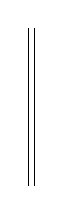
\begin{tikzpicture}\draw (0,0)--(0,2);\draw (.08,0)--(.08,2);\end{tikzpicture}}

Par dévissage, on est ramené au cas où $Y$ est une courbe. Supposons la d'abord complète, de sorte que $U+u\subset Y$ implique $Y+u\subset Y$ -- alors le résultat est bien connu. Ceci résulte p.ex. de la formule des pts fixes, qui implique que $\tau_u|_Y$ \inserted{si ce n'est l'identité,} a $2-2g$ pts fixes, ce qui (comme $g\geq2$ à cause de l'hypothèse anabélienne) est absurde.

Cela \deleted{signifie} \inserted{implique} donc, dans le cas général, \inserted{au moins si $g\neq1$,} que l'image de $u$ dans la partie abélienne de $J_Y^0(K)$ est nulle.

\margin{Si $g\geq2$, quitte à remplacer $Y$ par $\widehat Y$, OPS. $Y$ complète. Si $g=1$ ou 0, cf argument homologique plus bas}
\margin{\unsure{ne sert à rien ici}}

\deleted{[Or d'après la structure connue de $J_Y^0$ comme extension de $J_{\widehat Y}^0$ par un tore $\mathbb G_m^I/\mathbb G_m$ (où $I=\widehat Y-Y$) $u$ s'identifie à un élément de $(\mathbb G_m^I/\mathbb G_m)(K)$, donc est défini par $(\lambda_i)_{i\in I}$, les $\lambda_i\in k^*$, qui servent à construire un fibré inversible}
\margin{36}

\scanpage{38}
\deleted{sur la courbe ``pincée'' $Y'\deleted{\unsure{=\widehat Y/I|=\widehat Y\amalg_I}}$ déduite de $\widehat Y$ en contractant $I$ en un pt, en identifiant les fibres \inserted{réduites sur les $y_i\in I$} du faisceau inv. trivial sur $\widehat Y$, \deleted{\unsure{en}} à $k$ par les $\lambda_i$ -- donc entre elles. Alors $u+x$ (pour $x\in Y$) \inserted{de $J_Y^1$} est représenté par le faisceau $\underline O_{\widehat Y}[x]$ (associé au diviseur $x$), muni de ces $\unsure{\overline m}$s identifications.]}

Pour \inserted{que $x+u$} \deleted{qu'il} soit de la forme $y$ $(y\in Y)$ il faut déjà que $u+x$ et $y$ aient $\unsure{\overline m}$ image dans $J_{\widehat Y}^1$, ce qui \deleted{(pour un genre $g\geq1$)} \inserted{\unsure{si comme|comme} l'image de $u$ dans $J_{\widehat Y}^0$ est nulle,} implique déjà \inserted{(pour un $g\geq1$)} $x=y$, donc $u=0$. Si $g=0$, alors $r=\operatorname{card}I\geq3$ à cause de l'hyp. anabélienne, on \deleted{\unsure{remplace}} prend une partie \inserted{$J$,} de $I$ à deux éléments, et on remplace $\widehat Y$ par $\widehat Y\setminus J$ pour conclure encore à $x=y$ donc $u=0$.

\margin{Cependant, on ne sait pas que l'image de $u$ dans $J_{\widehat Y\setminus J}^0$ est nulle!}

[En fait, on a prouvé que si $u\in\operatorname{Ker}(J_Y^0-J_{\widehat Y}^0)$, alors $(Y+u)\cap Y=\varnothing$ -- et par ailleurs, s'il existe un ouvert non vide $U$ de $Y$ tel que $U+u\subset Y$, alors $u$ est dans le Ker précédent (\unsure{du moins si} $g\neq1$). Mais ces arguments ne marchent que pour \uline{$g\neq1$}.]
\margin{$g\geq2$?}

Il vaut mieux, dans le cas général, présenter les choses sous forme homologique. Considérons les deux \deleted{projections} \inserted{applications} $U\xrightarrow{i}Y$, don-
\margin{37}

\scanpage{39}
\mspage{19}
et $j:U-Y$ induit par $\tau_u$, je dis que $H_1(i)=H_1(j)$, ou ce qui revient au $\unsure{\overline m}$, puisque $Y\xrightarrow{\alpha}J_Y^1$ induit un iso. $H_1(\alpha):H_1(Y)-H_1(J_Y^1)$, que $H_1(\alpha)H_1(i)=H_1(\alpha)H_1(j)$, ou encore $H_1(\alpha i)=H_1(\alpha j)$.

Or on a $\alpha j=\tau_u(\alpha i)$ donc \deleted{il suffit de}
\[
H_1(\alpha j)=H_1(\tau_u)H_1(\alpha i)
\]
et on sait que $H_1(\tau_u)=\operatorname{id}$, OK. Cela étant, soit $I=\widehat Y\setminus Y$, $J=\widehat Y\setminus U$, de telle façon que $J\supset I$, et soit $f:\widehat Y\simeq\widehat Y$ déduit de $j:U\subset Y$ en passant aux complétés, donc \inserted{$f(U)=\widehat Y-f(J)\subset Y=\widehat Y-I$} \deleted{\unsure{que}} implique $f(J)\supset I$ i.e. $J\supset f^{-1}(I)$.

On voit que le passage de $H_1(U)$ à $H_1(Y)$, par bouchage de trous en $J\setminus I$, a pour noyau la \inserted{somme des} $L_j$ avec $j\in J\setminus I$, et pour la raison analogue le noyau de $H_1(U)-H_1(Y)$ induit par $j$ est la somme des $L_j$ avec $j\in J\setminus f(I)$, d'ailleurs les $L_j$ $(j\in J)$ de $H_1(U)$ sont $\simeq\widehat{\mathbb Z}$ (resp. $\widehat{\mathbb Z}'$ en car. $p>0$...) et le sous-$\widehat{\mathbb Z}$-module engendré est $\widehat{\mathbb Z}^{J}/\widehat{\mathbb Z}$ (diagonale), donc \deleted{si $\operatorname{card}J\geq3$,} les sous-modules engendrés par deux parties \inserted{$I,I'$} de $J$ distinctes de $J$, ne peuvent être égaux que si $I=I'$, ou $I$ et $I'$ de cardinal $\mu-1$ (où $\mu=\operatorname{card}J$)
\inserted{Mais ici quitte à rapetisser $U$, on peut supposer}
\margin{38}

\scanpage{40}
\inserted{que $\operatorname{card}I<\operatorname{card}J-1$ i.e. $\operatorname{card}(J\setminus I)=\operatorname{card}(Y\setminus U)>1$.}
\deleted{On est donc dans l'un des cas suivants}

\deleted{a) $f^{-1}(I)=I$ i.e. $I$ stable par $f$.}

\deleted{b)} Donc on voit que l'on doit avoir $f^{-1}(I)=I$ i.e. $I$ stable par $f$, ce qui montre que $\tau_u$ induit en fait un \uline{automorphisme} de $Y$.
\margin{\deleted{Remplaçant \unsure{$u$}}}

\deleted{que $Y$ est une courbe elliptique}

Alors en remplaçant $Y=\widehat Y\setminus I$ par $Y'=Y\cup i=\widehat Y\setminus I'$ $(I'=I-\{i\})$, on voit de $\unsure{\overline m}$ que $f$ induit un autom. de $Y'$ (cet argument marche dès que $Y'$ s'injecte dans sa jacobienne généralisée, ce qui \deleted{sauf le cas où $Y$ \unsure{est} de type $(0,\nu)$ \unsure{avec}} \inserted{est le cas grâce à l'hyp. anabélienne sur $Y$})

\deleted{\unsure{et}} donc $f$ induit l'identité sur $I$. Si le genre est $0$, on en conclut (puisque $\nu\geq3$) que $f$ est l'identité; \deleted{Reste le} Dans le cas du genre $1$, on en conclut au moins que l'image de $u$ dans $J_{\widehat Y}^0$ est égale à $1$, et on termine comme précédemment.

Ouf!
\margin{39}

\scanpage{41}
\mspage{20}
2. La question de pleine fidélité.

Soient $K,K'$ deux extensions de type fini de $\mathbb Q$ --- est-il vrai que tout $\Pi_{\mathbb Q}$-homomorphisme $\Pi_{K'}-\Pi_K$ provient d'un homomorphisme de corps $K'\longrightarrow K$? On est ramené aussitôt au cas où --- une clôture algébrique $\overline{\mathbb Q}$ de $\mathbb Q$ étant choisie, d'où un $\Gamma_{\overline{\mathbb Q}/\mathbb Q}$ --- $K$ et $K'$ ont des sous-corps $k,k'$ (clôture alg. de $\mathbb Q$ dans $K$ resp. $K'$) isomorphes, avec des \deleted{iso} \inserted{plongt} $k,\deleted{k'}\longrightarrow\mathbb Q$ de $\unsure{\overline m}$ image, \unsure{d'où} que $E_K$ et $E_{K'}$ peuvent être considérés comme des extensions d'un même groupe $\Gamma=\Gamma_{\overline{\mathbb Q}/k}$ par $\pi_K$ resp. $\pi_{K'}$. La question est alors si \uline{tout} hom. de $\pi_{K'}$ dans $\pi_K$ qui commute à l'action de $\Gamma$, est induit par un hom. $K\hookrightarrow K'$. Pour construire ce dernier, il faudrait donc avoir une idée comment reconstruire $K,K'$ à partir des extensions $E_K,E_{K'}$, ou encore à partir
\margin{40}

\scanpage{42}
des groupes \inserted{profinis} extérieurs avec opérations de $\Gamma$ dessus. Et on pressent que le th. 3 du \S\ précédent (appliqué notamment à $\mathbb P_K^1$ convenablement troué...) pourrait donner la clef d'une telle construction.

Bien \deleted{\unsure{en}} sûr, des homomorphismes extérieurs quelconques $\pi_{\overline{K'}}\longrightarrow\pi_{\overline K}$ n'auront pas de sens géométrique --- l'idée est que les opérations du groupe $\Gamma=\Gamma_{\overline{\mathbb Q}/k}$ dessus sont si draconiennes, qu'il n'est possible de trouver un hom. extérieur qui y commute que par voie géométrique --- par des plongements de corps. \unsure{Pour|Or} il est essentiel ici que le corps de base ne soit pas quelconque, mais un corps tel que $\mathbb Q$ (ou, ce qui revient manifestement au $\unsure{\overline m}$, une extension de type fini de $\mathbb Q$). Encore faut-il se borner aux hom. $\pi_{K'}-\pi_K$ dont on décrète d'avance que l'image soit ouverte --- sinon
\margin{41}

\scanpage{43}
\mspage{21}
prenant pour $\pi_{K'}$ le groupe unité (i.e. $K'=k$), on trouverait un hom. $K\longrightarrow k$ correspondant!

Il faut pour le moins, pour travailler à l'aise à partir d'homomorphismes $\pi_{K'}-\pi_K$ (au lieu de $E_{K'}-E_K$) supposer que le centralisateur dans $\pi_K$ de l'image de tt sous-groupe ouvert de $\pi_{K'}$ soit réduit à $(1)$ --- on dira que l'homomorphisme en question est \uline{anabélien} disons --- de telle façon qu'à partir de cet hom. (commutant à $\Gamma$) on reconstitue l'hom. d'extensions $E_K$ et $E_{K'}$, qui est l'objet vraiment essentiel. P. ex. si justement $K'=k$, donc $E_{K'}=\Gamma$, ce qui nous intéresse, ce ne sont pas les $\Gamma$-hom. de $\pi_{K'}=(1)$ (!) dans $\pi_K$, mais bien les \uline{sections} de $E_K$ sur $\Gamma$.

\uline{Question-conjecture} Soient $K,K'$ deux corps, extensions \inserted{de type} \unsure{finies|finie} de $\mathbb Q$, \deleted{considérons} \inserted{et} un morphisme $B_{K'}\longrightarrow B_K$ de topos sur $B_{\mathbb Q}$.
\margin{42}

\scanpage{44}
Les conditions suivantes sont-elles bien équivalentes

a) L'hom. provient d'un plongement de corps $K\subset K'$.

b) L'image \inserted{de l'hom. ext.} $E_{K'}\longrightarrow E_K$ a une image ouverte.

[c) L'hom. extérieur $E_{K'}-E_K$ est anabélien]
\margin{c) n'est pas assez fort, cf plus bas...}

\uline{NB} On sait que $a\Longrightarrow b\Longrightarrow c$, et que b) équivaut à $\pi_K-\pi_{K'}$ a une image ouverte.

Une réponse affirmative impliquerait que si $\deg\operatorname{tr}K'/\mathbb Q<\deg\operatorname{tr}K/\mathbb Q$, alors il n'y a pas de tel hom. $E_{K'}-E_K$, compatible avec les projections dans $E_{\mathbb Q}=\Gamma_{\mathbb Q}$, en particulier, \deleted{Toute section de} \inserted{il en résulterait} que \deleted{pour} toute section de $E_K$ sur $\Gamma=\operatorname{Im}(E_K-\Gamma_{\mathbb Q})$, ou sur un sous-groupe ouvert \inserted{$\Gamma'$} de $\Gamma$, a un centralisateur \inserted{non} trivial dans $E_K$ --- et comme son centralisateur dans $\Gamma$ est réduit à $(1)$, cela impliquerait que pour tte telle section, on aurait \inserted{(si $\pi_K\ne1$)} $\pi_K^{\Gamma'}\ne(1)$. Or je m'aperçois que
\margin{43}

\scanpage{45}
\mspage{22}
ceci est sans doute faux (cf plus bas \inserted{n\textsuperscript{o} 3}) --- il faudrait \inserted{\unsure{en}} \deleted{donc} \inserted{renforcer} c) ci-dessus en

c') L'hom. $E_{K'}^\circ-E_K$ induit par $E_{K'}-E_K$ est anabélien (où $E_{K'}^\circ$ est le noyau de l'hom. composé
\[
E_{K'}^\circ\longrightarrow\Gamma_{\overline{\mathbb Q}/\mathbb Q}\xrightarrow{\substack{\chi\ \text{caractère}\\\text{cyclotomique}}}\widehat{\mathbb Z}^{*}).
\]

Mais pour voir que cette condition est \uline{nécessaire} pour que l'hom. soit géométrique, il faudrait \deleted{savoir} vérifier que \inserted{pour} tout sous-groupe ouvert $E'$ d'un $E_K$, le centralisateur dans $E_K$ (non seulement de $E'$ lui-$\unsure{=|\overline m}$, mais même de $E'^\circ$) est réduit à $1$ --- ce qui résulte de la démonstration du th. 1, et du fait* que pour tt sous-groupe ouvert $\Gamma'$ de $\Gamma=\Gamma_{\mathbb Q}$, le centralisateur (non seulement de $\Gamma'$, mais $\unsure{=|\overline m}$) de $\Gamma'^\circ$ dans $\Gamma$ est réduit à $(1)$.
\margin{* à vérifier!}

Donc, la conjecture initiale ainsi corrigée donne la

\uline{Conséquence} (conjecturale) Pour toute \deleted{groupe de} section de $E_K$ sur \deleted{$\Gamma_{\mathbb Q}$, \unsure{soit}} \inserted{un sous-groupe ouvert $\Gamma'$ de $\Gamma_{\mathbb Q}$}, de sorte que $\Gamma'$ opère (effectivement) sur $\pi_K$, on a \inserted{(si $K$ pas alg. sur $\mathbb Q$ i.e. $\pi_K\ne(1)$)} $\pi_K^{\Gamma'^\circ}\ne(1)$.
\margin{44}

\scanpage{46}
À vrai dire, à certains égards les $\Gamma_K$ sont des groupes trop gros pour pouvoir travailler directement avec, il y a lieu de regarder $\Gamma_K$ comme un $\varprojlim$ de groupes $\Gamma_{U/\mathbb Q}$ associés à des modèles affines de $K$ --- et on s'intéressera plus particulièrement à des modèles affines qui sont des variétés élémentaires --- plus généralement, qui sont des $K(\pi,1)$ (au sens profini...). Il est possible qu'il faille d'ailleurs, dans l'énoncé de la conjecture de départ, prendre un hom. \inserted{ext.} $E_{K'}\longrightarrow E_K$ dont on suppose d'avance (en plus de l'hyp. anabélienne et de la compatibilité avec les hom. dans $\Gamma_{\mathbb Q}$) qu'elle est compatible avec les \uline{filtrations} de ces groupes, associées à ces modèles (``filtrations modéliques'' (grossières)).

Nous \unsure{allons} alors, en $\unsure{=|\overline m}$ temps que des extensions de t.f. de $\mathbb Q$, les hom. entre \unsure{elles|tels}, et
\margin{45}

\scanpage{47}
\mspage{23}
homomorphismes de groupes profinis associés, \deleted{regarder} \inserted{étudier} la situation analogue pour des ``modèles'' élémentaires\inserted{ anabéliens}, voire des modèles $K(\pi,1)$ généraux. (On peut aussi regarder des tels modèles sur un corps \deleted{\unsure{de nombres}} \inserted{$K$ ext.} de type fini de $\mathbb{Q}$ -- mais passons pour le moment sur cette situation mixte, un peu bâtarde\ldots) Si $U,V$ sont des tels modèles, tout morphisme $\unsure{V|U}\longrightarrow\unsure{U|V}$ définit un morphisme de topos galoisiens sur $B_{\mathbb{Q}}$, $B_U\longrightarrow B_V$, \deleted{\unsure{de tels}} et si $V$ est \deleted{anabélien} élémentaire anabélien, cet homomorphisme est connu quand on connaît seulement
\[
H_1(B_{\bar U},\mathbb{Z}_{\ell})-H_{\unsure{1}}(B_{\bar V},\mathbb{Z}_{\ell})
\]
-- ce qui est beaucoup moins que la classe d'iso. du hom. de $B_{\mathbb{Q}}$-topos. (En fait, \deleted{il suffit} \inserted{\unsure{sans hyp.}} anabélienne sur $V$, dès que $V$ est plongé dans une VA, $f$ est connu quand on connaît son action sur les \unsure{types|topos} étales\ldots). Mais quels sont les hom. $B_U\longrightarrow B_V$, ou $E_U\longrightarrow E_V$
\margin{46}

\scanpage{48}
qui correspondent à des morphismes de modèles ? Avec un peu de culot, on dirait

\uline{Conjecture fondamentale} : Soient $U,V$ deux schémas de t.f. sur $\mathbb{Q}$, \inserted{$V$ \deleted{\unsure{disjoint}} \unsure{supposé}} \unsure{réguliers|régulier}, $U$ une \deleted{modèle} \inserted{variété} élémentaire anabélienne sur une extension finie de $\mathbb{Q}$. \deleted{Alors} \inserted{Considérons} \deleted{tout hom.} \inserted{un hom.} $B_V\longrightarrow B_U$ des topos étales sur $\mathbb{Q}$ -- ou ce qui revient au même, un hom. de groupes extérieur
\[
f:E_V=\pi_1(V)\longrightarrow E_U=\pi_1(U),
\]
compatible avec les hom.\inserted{ ext.} dans $\Gamma_{\mathbb{Q}}=\pi_1(\mathbb{Q})$.
\margin{\uline{NB} \unsure{pr} l'instant \unsure{on se bornera surtout} au cas où $V$ lui-$\unsure{=|\overline m}$ est un modèle élémentaire anabélien, \unsure{disons} dim. $1$.}

Conditions équivalentes

 a) Cet hom. provient (à isom près) d'un homomorphisme $V\longrightarrow U$ sur les modèles (qui est alors uniquement déterminé)

 b) $f\mid E_V^\circ$ est anabélien, i.e. l'image par $f$ de $\forall$ sous-groupe ouvert de $E_V^\circ$ a un centralisateur réduit à $1$
\margin{47}

\scanpage{49}
\mspage{24}
Pour la nécessité de b), on est ramené aussitôt au cas où $V$ est réduit à un pt, où cela se réduit à la \deleted{``conséquence conjecturale'' de la \unsure{conjecture-question} préliminaire.}

\margin{\figure{\begin{tikzpicture}\draw (0,0)--(0,-4.3);\end{tikzpicture}}}
\uline{Conséquence conjecturale} Soit $\Gamma'\subset\operatorname{Im}(E_U\longrightarrow\Gamma_{\mathbb{Q}})$ un sous-groupe ouvert, correspondant à un corps $k$ fini sur $\mathbb{Q}$, considérons un $k$-point de $U$, d'où un relèvement $\Gamma'\longrightarrow E_U$, de sorte que $\Gamma'$ opère sur $\Pi_U$. Ceci posé, on a
\[
\Pi_U^{\unsure{\Gamma'^\circ}}=\{1\}.
\]

On étudiera par la suite les relations entre cette \inserted{cons.} ``conjecturale'', et la précédente (d'apparence opposée !) concernant les $E_K$.

La conjecture fondamentale sur les modèles implique la conjecture fondamentale sur les corps, à condition de prendre soin, dans cette dernière, de se limiter aux hom. compatibles aux filtrations modéliques,
\margin{et il \unsure{vaut mieux} se borner à l'équivalence de a) et b) -- les conditions c) sur les centralisateurs \unsure{risquent} de passer mal à la \uline{limite}.}

Plus généralement, prenant \inserted{\unsure{adaptés pour $U$}} des schémas, \deleted{de dim} qui sont des $\varprojlim$ de \deleted{schémas} \inserted{modèles élém.} \unsure{anabéliques|anabéliens}, avec morphismes de transition \inserted{des immersions ouvertes} affines
\margin{48}

\scanpage{50}
(pour pouvoir passer à la $\varprojlim$ dans la catégorie des schémas), pour $V$ un schéma $\varprojlim$ de schémas séparés réguliers de t.f. sur $\mathbb{Q}$ (morphismes de transition affines\inserted{ \unsure{imm. ouvertes}}, sans plus), Alors les morphismes \uline{dominants} de schémas $V\longrightarrow U$ doivent correspondre aux hom. ext $E_V\longrightarrow E_U$, compatibles avec les projections dans $E_{\mathbb{Q}}\simeq\Gamma_{\mathbb{Q}}$, et tels que l'image soit ouverte. P.ex. on pourrait prendre \inserted{pour} $U$, \deleted{$\operatorname{Spec}(\unsure{\mathcal{O}}_{X,x})$}, $V=$ les spectres d'anneaux locaux\inserted{ réguliers}, \unsure{ess.|ets.} de type fini sur $\mathbb{Q}$.

\figure{\begin{tikzpicture}\draw (0,0)--(.55,.03);\end{tikzpicture}}

Cette conjecture fondamentale (éventuellement revue et corrigée en cours de route !) étant admise, la question qui se pose ensuite est de déterminer les topos (pro) galoisiens sur $B_{\mathbb{Q}}$ qui proviennent de modèles élémentaires anabéliens -- ou encore, les $\Pi_U=\pi_1(\bar U)$ de tels modèles étant connus, de déterminer quelles sont
\margin{49}

\scanpage{51}
\mspage{25}
actions extérieures possibles des sous-groupes\inserted{ ouverts} $\Gamma$ de $\Gamma_{\mathbb{Q}}$ sur de tels groupes fondamentaux -- et éventuellement question analogue pour d'autres types de groupes profinis, correspondant à des $K(\Pi,1)$ qui se réaliseraient par des variétés algébriques (sur $\mathbb{C}$, disons), mais pas par des variétés élémentaires. (J'ai en vue avant tout des \deleted{topos} \inserted{variétés} modulaires, tels que, notamment, des variétés modulaires pour des courbes algébriques\ldots) À partir de là, on reconstruira par recollement, en termes profinis, tous les schémas lisses sur un corps de type fini sur $\mathbb{Q}$ (ou plutôt, la catégorie de ceux-là\ldots), ou plus gén. sur un corps quelconque -- puis, sans doute, par ``recollement'', la catégorie des schémas loc de type fini sur $\unsure{\forall}$ un $K$ -- tout au moins la cat. des fractions qui s'en déduit en \deleted{\unsure{égale}} rendant inv. les
\margin{50}

\scanpage{52}
homéomorphismes universels\ldots

Les réflexions précédentes suggèrent aussi des énoncés comme les suivants : Pour un schéma de base $S$ loc. noeth. donné, le foncteur $X\longrightarrow X_{\mathrm{et}}$, allant de la catégorie \deleted{réduits} des schémas\inserted{ réduits} loc. de prés. finie sur $S$, vers la 2-catégorie des \unsure{topos} au dessus de $X_{\mathrm{et}}$, est \deleted{pleinement} 1-fidèle (deux hom. $f,g:X\unsure{=|\rightrightarrows}Y$ tels que les homomorphismes\inserted{ $f_{\mathrm{et}},g_{\mathrm{et}}$} de topos $X_{\mathrm{et}}\rightrightarrows Y_{\mathrm{et}}$ au-dessus de $S_{\mathrm{et}}$ soient isomorphes, sont égaux) et $\unsure{=|\overline m}$ peut-être \uline{pleinement} \uline{fidèle}, quand on passe à la catégorie des fractions de $(\mathrm{Sch}_{\unsure{l.t.f.}})/S$ obtenue en rendant inv. les homéom. universels\ldots Expérimenter \deleted{\unsure{p}} ceci p.ex. pour les autom d'une courbe alg. propre sur une ext. finie de $\mathbb{Q}$, en \inserted{re}trouvant le ``fait'' que tout autom ext. de $E_K$ ($K$ le corps des fonctions de $X$) qui respecte la structure à \unsure{Qcts|Dcts} et qui commute à l'action de $\Gamma$, provient d'un autom de $X$
\margin{$S$ de car. $0$ ?}
\margin{51}

\scanpage{53}
\mspage{26}
3. \uline{Étude des sections de} $E_U$ \uline{sur} $\Gamma$.

Soit $U$ un \deleted{modèle élémentaire sur} \inserted{schéma connexe lisse de t.f. (\unsure{géométriquem.})} le corps $K$, d'où $E_U\longrightarrow E_K$, et on se propose d'étudier les sections mod $\Pi_{U/K}$ conjugaison --- plus généralement, on \unsure{veut} en $\unsure{=|\overline m}$ temps regarder les sections $E'_K\longrightarrow E_U$, où $E'_K$ est un sous-groupe ouvert de $E_K$. Ce qui signifie que l'on fait une extension de base finie sur $K$). Si \inserted{$K$ de type fini sur le corps $\mathbb{Q}$ et si} $U$ se plonge dans un schéma \deleted{abélien} \inserted{\unsure{ou} un groupe commutatif \deleted{\unsure{algébrique}} rigide}, l'application
\[
U(K)\longrightarrow \inserted{\text{Classes d'isomorphisme}}\ \text{Sections de }B_U\text{ sur }B_K
\]
i.e. classes de $\Pi_{U/K}$ conjugaison des sections de $\unsure{B_U|E_U}$ sur $\unsure{B_K|E_K}$

est injective. On va examiner d'autres façons \inserted{``géométriques''} de trouver des sections.

Supposons d'abord que $U$ est une courbe algébrique, \deleted{\unsure{qui a $\pi_1$ nul}} \inserted{qui ne soit pas de} type $(0,0)$ ou $(0,1)$ i.e. $\pi_1(\bar U)=\Pi_{U/K}\ne\{0\}$ ; Alors \unsure{on a pour} $\forall\ i\in\widehat U\setminus\bar U$ (``pt à l'infini''), le groupe de lacets $L_i$ fournit un scindage (au moins si $i$ est $/K$ i.e. \unsure{fixé}

\margin{On a choisi un rev. universel $\widetilde U$ de $U$ pour définir $\bar K$, et $E_U,E_{\unsure{K}}$, et $E_U\longrightarrow E_K$}
\margin{(1)\diagram{\begin{tikzcd}[ampersand replacement=\&,row sep=small]
1\\
E_K=\Gamma\arrow[u]\\
E_U\arrow[u,no head]\\
\Pi_{U/K}\arrow[u]\\
1\arrow[u]
\end{tikzcd}}}
\margin{52}

\scanpage{54}
par $E_{\bar K/K}$) en prenant son centralisateur $Z(L_i)$ dans $E$, d'où
\[
(2)\qquad
\diagram{\begin{tikzcd}[ampersand replacement=\&,column sep=small]
1\arrow[r,no head]\&L_i\arrow[r,no head]\arrow[d,phantom,"\simeq" description]\&Z(L_i)\arrow[r]\&\Gamma\arrow[r]\&1\\
\&T_\infty(\bar K^*)=T\&\&\&
\end{tikzcd}}
\]
et on prend les scindages de cette extension. Il en existe, p.ex. définis par une uniformisante de $\unsure{\mathcal O}_{\widehat U,i}$. L'ens des classes de conjugaison des \deleted{\unsure{ses}} scindages \deleted{\unsure{les}} de (\unsure{1|2}) est un torseur sous \deleted{$H^1(\Gamma,T)$}
\[
(3)\qquad H^1(\Gamma,T)\simeq\varprojlim_n H^1(K,{}_n\mu)\simeq\widehat{K^*}=\varprojlim_n K^*_n
\]
et \deleted{\unsure{cet ensemble}} s'envoie injectivement \deleted{\unsure{vers}} dans l'ens des classes de $\pi$-conj. de scindages.

\uline{Proposition} On suppose $(g,\nu)\ne(0,0),(0,1)$ i.e. $\Pi_{\bar U}=\Pi_{U/K}\ne(1)$. Alors les classes de \inserted{$\pi$-conjugaison} scindages \deleted{\unsure{assoc.}} de (1) définis par les scindages de (2) sont distinctes de celles associées aux pts de $U(K)$. \deleted{De plus,} Si \inserted{(en plus)} $(g,\nu)\ne(0,2)$, \deleted{\unsure{dans le}} \inserted{i.e. si on est} dans le cas anabélien, alors les classes de $\pi$-conjugaison de scindages de (1), associés à des scindages de (2) pour deux indices $i\deleted{\unsure{a}}=i_1$ et $i=i_2$ distincts \inserted{sont distinctes.}
\margin{C'est démontré sauf pour le type $(0,3)$, qui mérite un examen approfondi.}
\margin{53}

\scanpage{55}
\mspage{27}
La première assertion s'obtient en ``bouchant'' le trou $i$, alors la section envisagée devient la section de $U\cup\{i\}=U'$ associée au pt $i$, et elle est donc distincte de celle associée aux \deleted{pts} autres pts de $U'$, i.e. aux pts de $U$ --- a fortiori avant de passer au quotient par le ss-groupe inv. engendré par $L_i$. On \unsure{voudra} de $\unsure{=|\overline m}$ façon se convaincre que les classes de conj. des scindages associés à un $L_{i_1}$ et un $L_{i_2}$, $i_1\ne i_2$, sont distinctes --- ça marche dans tous les cas sauf le cas du type $(0,3)$, \deleted{\unsure{car}} car en bouchant deux trous on tombe sur le type $(0,1)$, où on ne dispose pas du résultat d'injectivité. Mais on peut s'en tirer autrement, à condition d'admettre que pour un scindage de (2), faisant opérer $\Gamma$ sur $\pi$, on a
\[
(3)\qquad\pi^{\Gamma^\circ}=L_i
\]
(donc $\pi^\Gamma=(1)$, d'ailleurs) --- résultat qui me paraît hautement plausible. Cela
\margin{À énoncer parmi les conjectures-clefs\ldots}
\margin{54}

\scanpage{56}
montrerait que la classe de conjugaison des sections détermine la classe de conjugaison de $L_i$, donc $i$.

\uline{Conjecture A} Soit $U$ courbe alg. anabélienne géom. connexe sur corps $K$ de type fini sur $\mathbb{Q}$. Alors toute section de (1) est \deleted{définie} d'un des deux types précédents, i.e. soit définie par un pt de $U(K)$, soit par une section d'une extension (2), avec $i\in I(\bar K)^\Gamma$ i.e. un pt de $\widehat U\setminus U$, rationnel sur $K$.
\margin{Il y a \uline{\unsure{de plus}} les précisions $\pi^{\Gamma^\circ}=(1)$ (premier cas) $\pi^{\Gamma^\circ}=L_i$ (deux. cas)}

Si on admet cette conjecture, alors on en conclurait, par passage à la limite, en considérant le corps des fonctions $L$ de $U$ et $E_L\longrightarrow E_K$ ($E_L$ peut être considéré comme un groupe à lacets ``infini'' car une infinité de \inserted{classes de} ss-groupes lacets\inserted{ $L_i$}\ldots) que tout scindage de cette extension provient d'un scindage d'une extension du type (2), avec $i\in I^\Gamma=X(K)$ ($X=\widehat U$). Les classes de tels scindages
\margin{55}

\scanpage{57}
\mspage{28}
se grouperaient donc \deleted{dans de} par paquets (en regardant les centralisateurs des ss-groupes images de $\Gamma^\circ$ par ses sections,\deleted{)} et en mettant ensemble des scindages qui ont des $\unsure{\mathrm{Zentr}}(\Gamma^\circ)$ conjugués (même s'ils ne sont eux-mêmes conjugués). Donc on \unsure{retrouve} encore une description de $X(K)$ (donc aussi des $X(K')$ pour $\forall$ ext. finie \inserted{$K'$} de $K$) en termes de l'extension $E_L$ de $E_K$ par $\Pi_{L/K}$, en $\unsure{=|\overline m}$ temps qu'une façon de reconstituer les $U=X\setminus\bar I$\ldots Donc en fait c'est la structure $E_L\longrightarrow E_K$ qui est la plus riche a priori, et de loin plus commode pour le genre $0$ et $1$, où la considération des $U$ de type $(g,\nu)$, $(2g+\nu\geq3)$ casse le groupe ``continu'' d'automorphismes\ldots La forme ``modélique'' de la conjecture précédente revient à la forme ``birationnelle'', quand on y précise cette dernière en disant que \unsure{tt}
\margin{56}

\scanpage{58}
scindage de $E_U-E_K$ se remonte en un scindage de $E_L-E_K$ (ou aussi, \deleted{par} en un scindage de $E_V-E_K$, si $V$ est un modèle $\subset U$)

On va mettre les conjectures précédentes (sous forme modélique, disons) sous une forme plus géométrique, en introduisant, en $\unsure{=|\overline m}$ temps qu'un revêtement universel \deleted{\unsure{de}} $\widetilde U$ de $U$, le normalisé \deleted{de} $X'$ de $X$ dans $\widetilde U$ (où $X=\widehat U$). (NB je m'abstiens de le noter $\widetilde X$, car que justement il n'est pas étale sur $X$\ldots). Notons que pour $i\in\bar I=\bar X-\bar U$, les \inserted{l'ens des} $L_i$ de $\bar\pi=\pi(\bar U)$ sont en corr. $1-1$ avec l'\deleted{ens} fibre $X'_i$ de $X'$ au dessus de $i$

\diagram{\begin{tikzcd}[ampersand replacement=\&,column sep=large,row sep=large]
X\arrow[r,no head]\arrow[d,phantom,"\cup" description]\&\bar X\arrow[r,no head]\arrow[d,phantom,"\cup" description]\&X'\arrow[d,phantom,"\cup" description]\\
U\arrow[r,no head]\arrow[d,no head]\&\bar U\arrow[r,no head]\arrow[d,no head]\&\widetilde U\\
K\arrow[r,no head]\&\bar K\&
\end{tikzcd}}

Donc $X'$ peut être considéré comme la réunion de $\widetilde U$, et de $X'|\bar I=$ ensemble des sous-groupes lacets de $\bar\pi$, qui apparaissent ainsi comme des ``pts à l'infini'' du rev. universel $\widetilde U$. D'ailleurs $E_U$ s'inter-
\margin{57}

\scanpage{59}
\mspage{29}
prète comme le groupe \inserted{\unsure{topologique|topologisons}} des $U$-autom du schéma $\widetilde U$, et $E_U\longrightarrow E_K$ comme l'hom de passage au quotient induit sur $\bar K$, identifié à la clôture alg. de $K$ dans $H^0(\widetilde U,\mathcal O_{\widetilde U})$, donc $E_U$ opère sur $\operatorname{Spec}\bar K$ de façon naturelle. Une section de $E_U$ sur $E_K$ est donc une action de $E_K$ sur $\widetilde U$, compatible avec son action sur $\unsure{\widetilde U|\bar U}$, et continue dans un sens convenable (sans doute la conv. \unsure{simple-discrète} sur les \deleted{$\unsure{\widetilde U_i}$} $\bar U_i$ finis sur $\bar U$ entre $\widetilde U$ et $\bar U$\ldots).

Considérons alors la

\uline{Conjecture B} Toute telle action de $\Gamma$ sur $\widetilde U$ admet \uline{dans $X'$}$=\widehat{\widetilde U}$ un pt fixe et un seul.
\margin{\figure{\begin{tikzpicture}\draw (0,0)--(0,-3.1);\end{tikzpicture}}}
\margin{et $\unsure{=|\overline m}$ l'action induite de $\Gamma^\circ$ doit avoir un pt fixe et un seul --- cf plus bas.}

Ceci signifie donc

a) S'il y a un pt fixe à distance finie i.e. $\widetilde x\in\widetilde U^\Gamma$, alors 1°) L'image de $\widetilde x$ dans $U$ est uniquement déterminée --- c'est essentiellement le \unsure{th.3} du $\S1$ (deux pts distincts de $U(K)$ définissent des classes de conj. de scindages distinctes) et
\margin{58}

\scanpage{60}
2°) $\pi^\Gamma=(1)$ (i.e. il n'y a pas d'autres pt fixes dans $\widetilde U$ sur le $\unsure{=|\overline m}$ $x\in U(K)$), et enfin

3°) il n'y a pas en $\unsure{=|\overline m}$ temps de pt fixe $\unsure{\widetilde x}$ à l'infini --- i.e. il n'existe pas de $L_i$ normalisé par $\Gamma$, i.e. un scindage du premier type n'est pas en $\unsure{=|\overline m}$ temps du deuxième (fait que nous avons établi directement, précédemment).

\margin{C'est une particularisation d'une ``conséquence conjecturale'' de la conjecture du $\S1$ --- sauf qu'il faudrait écrire $\pi^{\Gamma^\circ}=(1)$}

D'autre part, dans le cas de pts fixes à l'$\infty$, l'unicité de l'image dans $X$ signifie qu'une $\unsure{=|\overline m}$ action effective ne peut normaliser à la fois un $L_i$ et un $L_j$ ($i\ne j$) --- fait également établi sauf dans le cas $(g,\nu)=(0,3)$ --- et l'unicité --- au dessus d'un $i\in\bar I$ fixé signifie que le $L_i$ \inserted{($i$ fixé)} normalisé par $\Gamma$ est unique, ce qui est un affaiblissement de la relation $L_i=\deleted{\unsure{Z_\pi|Z_{\mathrm{en}}}}\pi^{\Gamma^\circ}$ pour ces opérations, conjecturée plus haut.
\margin{59}

\scanpage{61}
\mspage{30}
En fait, je conjecture que dans la conj. B, il est $\unsure{=|\overline m}$ vrai que $\Gamma^\circ$ agissant sur $X'=\widehat{\widetilde U}$ a un pt fixe et un seul (ce qui est plus fort, que ce point \inserted{fixe} sera nécessairement fixe par $\Gamma$). Ceci \deleted{signifie}\inserted{implique}, dans le cas des pts fixes à distance finie, qu'on a alors $\pi^{\Gamma^\circ}=(1)$, comme il se devrait en général --- et dans le cas du pt fixe à l'infini, que
\[
\pi^{\Gamma^\circ}\subset\operatorname{Norm}_{\pi}(L_i)=L_i
\]
donc la relation $\pi^{\unsure{\Gamma_0|\Gamma^\circ}}=L_i$ ``hautement plausible'' de tantôt !

Du coup je me demande d'ailleurs si ces énoncés ne devraient pas être valables sans partir d'une action de $\Gamma$ \deleted{\unsure{tt}} entier, mais seulement de $\Gamma^\circ$ (ou d'un sous-groupe contenant un sous-groupe ouvert de $\Gamma^\circ$, plus gén.) --- ce qui signifierait plus ou moins que
\margin{60}

\scanpage{62}
tous nos beaux énoncés devraient être valables, non seulement pour un corps de base $K$ ext. de type fini de $\mathbb{Q}$, mais dès que $K$ est ext. de type fini d'un corps cyclotomique (pas néc. fini sur $\mathbb{Q}$).

Nous pourrions définir les \uline{courbes de Poincaré} sur un corps alg. clos $\bar K$ de car. $0$ comme étant les courbes isomorphes à des rev. universels de courbes alg. anabéliennes sur $\bar K$ (deux courbes anabéliennes $\unsure{=}\ \bar U,\bar V$ sur $\bar K$ définissent des rev. de Poincaré isomorphes, ssi $\exists$ un revêtement fini étale de l'une, isomorphe à un rev. fini étale de l'autre\ldots).

Étant donné une courbe de Poincaré $\widetilde{\unsure{\mathcal U|U}}$ sur $\bar K$, \deleted{telle} on définit canoniquement sa complétée\inserted{ $\widehat{\unsure{\mathcal U|U}}$}, de telle façon que $\forall$ autom de $(\widetilde{\unsure{\mathcal U|U}},\bar K)$ (pas néc. induisant l'identité sur $\bar K$) induise un autom. de $\widehat{\unsure{\mathcal U|U}}$.
Ceci posé :
\margin{61}

\scanpage{63}
\mspage{31}
\uline{Conjecture B'} Soit $K$ un corps de type fini sur $\mathbb{Q}$ (ou sur un corps cyclotomique, cela suffira peut-être), $\bar K$ une clôture algébrique de $K$, $\mathcal U$ une courbe de Poincaré sur $\bar K$, de complétée $\widehat{\mathcal U}=\mathcal X$. Considérons une action de $\Gamma=\Gamma_{\bar K/K}$ sur $\mathcal U$, compatible avec son action sur $\bar K$, d'où une action de $\Gamma$ sur $\mathcal X$. Ceci posé :

il existe un point fixe et un seul de $\Gamma^\circ$ agissant sur $\mathcal X$

($\Gamma^\circ$, noyau du caractère cyclotomique $\Gamma\xrightarrow{\chi}\widehat{\mathbb Z}^{\!*}$).

La différence avec la conjecture B, que celle-ci renforce, c'est qu'ici on ne suppose \uline{pas} que l'action de $\Gamma$ sur $\mathcal U$ normalise l'action d'un groupe profini $\pi$, agissant librement sur $\mathcal U$ de façon \unsure{que|q.} $\mathcal U/\pi$ soit une courbe alg. anabélienne sur $\bar K$.
\margin{62}

\scanpage{64}
Que deviendraient les conjectures précédentes, quand on les applique à une situation où $K$ est remplacé par un modèle $S$ de $K$ (disons, élémentaire anabélien), quand $U_K$ provient d'une courbe relative $U_S$ sur $S$ — de sorte qu'on a un hom de groupes
(4)\quad\diagram{\begin{tikzcd}[ampersand replacement=\&]E_{U_S}\arrow[d]\\E_S\end{tikzcd}}
de noyau $\pi_{\bar U}$, dont $E_{U_K}-E_K$ est déduit par chgt de base i.e. par produit fibré
(4')\quad\diagram{\begin{tikzcd}[ampersand replacement=\&]
\pi \arrow[r,equal] \arrow[d] \& \pi \arrow[d] \\
E_{U_S} \arrow[d] \& E_{U_K} \arrow[l] \arrow[d] \\
E_S \& E_K \arrow[l,"\mathrm{surj}"'] \arrow[ul,dashed,"\varphi"']
\end{tikzcd}}
Ainsi, les sections de $E_{U_K}$ sur $E_K$ correspondent aux \deleted{\uline{\unsure{fausses|bonnes}} sections de} \inserted{relèvements continus} $E_K\longrightarrow E_{U_S}$ de l'hom surjectif $E_K\longrightarrow E_S$, et parmi ces relèvements, ceux qui sont \deleted{\unsure{nuls}}\inserted{triviaux} sur le noyau de $E_K\longrightarrow E_S$ correspondent exactement aux sections
\margin{63}

\scanpage{65}
\mspage{32}
de $E_{U_S}$ sur $U_S$. Nos conjectures impliquent donc qu'il y a exactement deux sortes de telles sections : 1°) celles qui correspondent à des pts de $U_K/K$ i.e. à des sections rationnelles de $U_S$ sur $S$ — mais on va vérifier sans mal, sans doute, qu'une telle section rationnelle ne correspond effectivement à une section de \inserted{l'extension} (4), que si c'est une section \deleted{rationnelle} régulière (à vérifier tantôt). 2°) Celles correspondant à des $i\in I(U_{\bar K})$ rationnels sur $K$, i.e. à une \uline{section} de $\widehat U_S\setminus U_S=S'$ (étale fini sur $S$) sur $S$. Et il faudrait étudier encore à quelles conditions une telle section définit un paquet non vide de scindages de (4) — et comment déterminer exactement tous ces scindages.

Avant d'élucider ces deux points, un peu techniques, je voudrais voir
\margin{64}

\scanpage{66}
dans quelle mesure la conjecture A (ou B) faite dans ce §, permet de reconstruire la catégorie des modèles élém. anabéliens sur $Q$, \inserted{et} celle des extensions de type fini de $Q$ et des modèles élém. anabéliens sur ceux-ci, en termes des groupes extérieurs \inserted{(ou top. \unsure{galoisiens})} associés à partir bien sûr de la donnée fondamentale de $\Gamma_Q=\Gamma_{\bar Q/\bar Q_0}$, opérant extérieurement sur $\widehat\pi_{03}$, d'où déjà l'extension $E_{03}=E_{U_{03}/Q}$, où $U_{0,3}=\mathbb P^1_Q-\{0,1,\infty\}$.

Prenons les \inserted{classes de $\widehat\pi_{03}$-conj. de \unsure{scissions|sections}} sections de $E_{03}$ sur $\Gamma_Q=\Gamma$ \inserted{telles que le centralisateur de $\Gamma^\circ$ soit trivial (sections ``admissibles'')}, i.e. les ``points'' \deleted{\unsure{de}} \inserted{\unsure{(ou les sections)|(ou les points)} du} topos $B_{\widehat\pi_{0,3},\Gamma_Q}^{\unsure{\sharp}}$ sur $B_{\Gamma_Q}^{\unsure{\sharp}}$ — on trouve un ensemble sur lequel $\Gamma$ opère (qui n'est autre que $U_{03}(\bar Q_0)$, à \unsure{deux} cas. près). Pour tout ens. fini \inserted{$I$} de sections, \inserted{stable par $\Gamma$,} le foncteur
\margin{65}

\scanpage{67}
\mspage{33}
``forage de trous'' doit nous fournir un groupe extérieur $\Pi_{0,3}(I)$, \inserted{de type $(0,3+\operatorname{card} I)$,} sur lequel $\Gamma$ opère (il vaut mieux peut-être utiliser le yoga introduit par ailleurs des groupoïdes rigides — donc on \unsure{peut|pourra} \unsure{ou devra} aussi boucher certains des trous $0,1,\infty$ — on trouve donc l'équivalent groupoïdal de la \deleted{``sphère \unsure{ar.}} droite projective $\mathbb P^1_Q$, on l'appelle la sphère arithmétique — qui correspond à un groupe \inserted{ext.} à lacets infini sur lequel $\Gamma$ opère — en fait, ce n'est autre que $E_{K_1}$, où $\unsure{\vert}$
\[
\tag{6}K_1=Q(\deleted{\unsure{X_1|x_1}}\,T_1)
\]
est l'extension transcendante pure \inserted{typ.} de degré $1$ de $Q$.

Partant de (6), on construit de $\unsure{\overline m}$ l'équivalent groupoïdal de $\deleted{\unsure{X|P}}\,U_{0,3}$ $\unsure{\longleftarrow}$ et on remonte comme
\margin{66}

\scanpage{68}
précédemment, pour avoir, soit des courbes de type $(0,\nu_2)$ sur $K_1$\unsure{,} (ou sur une extension finie de $K_1$) soit des courbes relatives de type $(0,\nu_2)$ sur une courbe sur $Q$ \deleted{de type} (ou une extension finie de $Q$, ou un rev. \deleted{étale} étale fini d'une telle $U_{0\nu_1}$).

On procède de proche en proche pour construire \unsure{finalt} tous les $E_K$ sur $\deleted{\unsure{E}}\,E_Q$ (car tt corps ext. de type fini de $Q$, est ext. finie d'une ext. transcendante pure) et tous les modèles élémentaires, où à chaque cran la fibration est soit une courbe de genre $0$, soit un rev. étale fini d'une telle fibration particulière. Sauf erreur, ça fait assez pour avoir un syst. fondamental de voisinages de tt point d'un $X$ lisse sur un $K$.
\margin{67}

\scanpage{69}
\mspage{34}
et de reconstituer en principe les schémas lisses sur des $K$, par recollements de tels morceaux avec des ``imm. ouvertes''. Mais je sens nettement que pour faire une telle description, il me faudra développer un langage géométrique qui colle mieux à l'intuition géométrique, que les sempiternelles extensions de groupes profinis\ldots\ ou actions extérieures, et où les points rigides (à coeff dans des clôtures algébriques de corps) jouent un rôle prépondérant. Il \deleted{me} faudra y revenir dessus -- et en même temps, expliciter les topos étales (pas seulement le ``morceau $K(\pi,1)$) tout entiers des schémas décrits ici par des extensions.
\margin{68}

\scanpage{70}
Reprenons le cas de $U=U_S$ schém. relatif sur $S$, ``élémentaire'' sur $S$ -- à fibres successives anabéliennes (s'il le faut) ou des courbes à $\pi_1$ non nul, $S$ étant lui-$\unsure{\overline m|\overset{m}{=}}$ (pour fixer les idées) lisse sur $\mathbb{Q}$, irréductible, corps de fonctions $K$, et reprenons le diagramme 5. Considérons une section rationnelle \inserted{$f$} de $U$ sur $S$, définissant une section de $E_{U_{\unsure{\eta|K}}}$ sur $E_K$ -- ou, ce qui revient au même, un relèvement de l'hom surjectif $E_K\longrightarrow E_S$ en $E_K\longrightarrow E_{U_S}$ \inserted{(composé de \inserted{la section} $E_K-E_{U_{\unsure{\eta|K}}}$ avec $E_{U_{\unsure{\eta|K}}}-E_{U_S}$)}. Je veux montrer que $f$ est partout défini i.e. une \unsure{section} \deleted{\unsure{rationnelle}} de $U_S$ sur $S$, ssi la section de $E_{U_{\unsure{\eta|K}}}$ sur $E_K$ provient d'une section de $E_{U_S}$ sur $E_S$, i.e. ssi le relèvement $E_K\longrightarrow E_{U_S}$ s'annule sur
\margin{69}

\scanpage{71}
\mspage{35}
le noyau de $E_K\longrightarrow E_S$.

Notons que cette dernière condition est une condition ``de codimension 1 sur $S$'' -- de façon plus précise, si $Z$ est un sous-schéma fermé de $S$ de codim $\geq 2$, \deleted{alors} alors, posant $S'=S\setminus Z$, on a $\pi_1(S')\xrightarrow{\sim}\pi_1(S)=\unsure{E}_S$ par le ``théorème de pureté'' -- donc le noyau de $\deleted{\unsure{\pi_1}}E_K\longrightarrow E_S$ est le $\unsure{\overline m|\overset{m}{=}}$ que celui de $E_K-E_{S'}$, ou, si on préfère (comme $S'$ n'est pas un ``modèle'') que le sous-groupe \deleted{\unsure{nor-}}\inserted{fermé} engendré par les noyaux des $E_K\longrightarrow E_{S'_i}$, où les $S'_i$ sont des ouverts ``modèles'' qui recouvrent $S'$. Si donc la condition envisagée est remplie relativement aux $S'_i$ (qui pour-\deleted{\unsure{tant}} ne recouvrent pas $S$, seulement $S'$) -- ce qui est censé signifier que la section
\margin{70}

\scanpage{72}
rationnelle envisagée est morphique sur les $S'_i$, i.e. sur $S'$ -- alors elle est vérifiée relativement à $S$ -- ce qui est censé signifier que la section est morphique sur $S$. Donc, pour se rassurer, il faudrait s'assurer a priori qu'une section de $U_{S'}$ sur $S'$ se prolonge automatiquement en \deleted{$U$} une section de $U_S$ sur $S$. De proche en proche, on est ramené au cas d'une courbe relative $U_S=X_S-T$, $X$ lisse \inserted{sur $S$} de dim. relative 1, $T$ fini étale sur $S$, \deleted{\unsure{le}} \unsure{OPS|\deleted{pas}} $\unsure{\overline m|\overset{m}{=}}$ $T$ décomposé sur $S$. Si $X$ de genre relatif $\geq 1$, on sait (th. de Weil) que la section se prolonge en une section de $X$, soit $D$ l'image inverse de $T$, c'est un diviseur sur $S$, dont la trace sur $S'=S\setminus Z$ est nul, donc (comme $\operatorname{codim}(Z,S)\geq\unsure{1|2}$) il est nul, OK.
\margin{71}

\scanpage{73}
\mspage{36}
\[
(9)\qquad\diagram{\begin{tikzcd}[ampersand replacement=\&,column sep=small]
U_S \arrow[r,no head] \arrow[d,no head] \& U_{O_x} \arrow[r,no head] \arrow[d,no head] \& U_K \arrow[r,no head] \arrow[d,no head] \& U_{\overline K} \arrow[r,no head] \arrow[d,no head] \& \widetilde U_S \\
S \arrow[r,no head] \& \underline O_x \arrow[r,no head] \& K \arrow[r,no head] \& \overline K \&
\end{tikzcd}}
\]
\[
(10)\qquad\diagram{\begin{tikzcd}[ampersand replacement=\&]
E_{U_S} \arrow[d] \& E_{U_{O_x}} \arrow[l] \arrow[d] \& E_{U_K} \arrow[l] \arrow[d] \\
E_S \& E_{\underline O_x} \arrow[l] \& E_K \arrow[l] \arrow[ul,dashed,"\varphi_x"]
\end{tikzcd}}
\]
avec des carrés cartésiens, et des flèches horizontales surjectives. L'hom $E_K\longleftarrow E_{U_S}$ est composé d'un relèvement $E_K-E_{U_{O_x}}$ de $E_K\longrightarrow E_{O_x}$, avec l'hom canonique $\unsure{\widehat E}_{U_{O_x}}-E_{U_S}$. (Les \inserted{\deleted{derniers}} relèvements $E_K\longrightarrow E_{U_{O_x}}$ correspondent biuniv.$^{\mathrm t}$ aux sections de $E_{U_\eta}$ sur $E_K$, ou aux relt$^{\mathrm s}$ de $E_K-E_S$ en $E_K-E_{U_S}$\ldots)

Ceci dit, j'ai envie de prouver que $\varphi_x:E_K\longrightarrow E_{U_{O_x}}$ s'annule sur $I_x$, i.e. provient d'une section de $E_{U_{O_x}}$ sur $\underline O_x$ sss la section rationnelle correspond$^{\mathrm t}$ * de $U_S/S$ est définie en $x$. Ceci implique
\margin{\uline{NB} Le quotient de $E_K$ par le \unsure{s.groupe} engendré par $\unsure{I_x|\overline I_x}$ n'est autre que $E_{\underline O_x}=\pi_1(\operatorname{Spec}\unsure{O_x})$}
\margin{72}

\scanpage{74}
l'assertion précédente (que la section $\unsure{\psi|\varphi}$ de $E_{U_\eta}$ sur $E_K$ provient d'une section de $E_{U_S}$ sur $E_S$, sss la section rationnelle correspondante est morphique)

Mais il s'agit ici d'un énoncé en fait purement géométrique, que j'ai envie de reformuler sous forme plus générale :

\uline{Théorème.} \deleted{\unsure{2|3}}\unsure{(?)} Soit $\unsure{S|T}$ un trait (spectre d'un anneau-jauge), $U$ un schéma relatif ``élémentaire'' sur $T$, anabélien*, $K$ le corps des fonctions de $T$, On choisit un rev. universel $\widetilde U$ de $U$, d'où une clôture alg. $\overline K$ de $K$, et on considère l'extension
\[
E_U=\pi_1(U;\widetilde U)\quad\text{de}\quad E_K=\pi_1(K,\overline K)\simeq\operatorname{Gal}(\overline K/K)
\]
par $\pi=\pi_1(U_{\overline K},\widetilde U)$. \deleted{Considérons une} \inserted{On a donc} \deleted{section pt $K$-rationnel de $U_K$,} \inserted{un carré cartésien de groupes profinis}

\uline{d'où}
\[
\diagram{\begin{tikzcd}[ampersand replacement=\&]
E_U \arrow[d,"\mathrm{surj}"'] \& E_{U_\eta} \arrow[l,"\mathrm{surj}"'] \arrow[d,"\mathrm{surj}"] \\
E_S \& E_K=\operatorname{Gal}(\overline K/K) \arrow[l,"\mathrm{surj}"]
\end{tikzcd}}
\]
où $E_S$ s'identifie au quotient de $E_K$ par le sous-groupe nor. fermé engendré par un groupe
\margin{* anabélien est inutile -- il suffit que les fibres de dim 1 des fibrations élémentaires de $U$ ne soient pas des types $(0,0)$ ou $(0,\unsure{1})$ -- i.e. à $\pi_1$ nul}
\margin{73}

\scanpage{75}
\mspage{37}
d'inertie $I_x=T_\infty(\overline K)$, cf plus haut. Soit $f_K$ $\unsure{K}$ un pt de $U_K$ rat/$K$, d'où une section $\psi=\psi_{f_K}$ de $E_K$ sur $E_{U_K}$. Ceci posé les conditions suivantes sont équivalentes

\noindent a) $f_K$ se prolonge en une section de $U$ sur $S$

\noindent b) $\psi$ provient d'une section de $E_U$ sur $E_S$

\noindent b') le composé $E_K\xrightarrow{\psi}E_{U_K}\longrightarrow E_U$ s'annule sur $I_x$

\deleted{\unsure{c)}}

L'équivalence de b) et b'), et qu'ils soient impliqués par a), est clair. C'est l'implication $\mathrm{b)}\Longrightarrow\mathrm{a)}$ qui demande une démonstration. On est ramené aussitôt, par descente, au cas \deleted{\unsure{d'un}} où $T$ est strictement local (donc $E_K=\operatorname{Gal}\overline K/K$ est réduit à son ss-groupe d'inertie, \inserted{et $E_S=(1)$}). On est ramené de proche en proche au cas où $U/S$ est une courbe relative élémentaire, \deleted{de genre $g\geq 1$,} \inserted{$U=X\setminus T$, $X$ lisse et propre.} Alors $f$ se prolonge en une section $f$ \deleted{rationnelle}\inserted{de} $X$ sur $S$, et la conclusion est que $f(S)\subset U$. Donc on est ramené finalement au

\uline{Lemme} Soit $X$ schéma projectif lisse de dim relative 1 connexe sur $\unsure{S|T}$ trait strictement local,
\margin{74}

\scanpage{76}
Soit $T\subset X$ sous schéma, fini étale sur $S$, donc $T\simeq I_S$, $I$ ensemble fini, et soit $U=X\setminus T$ (donc $T$ est défini par une famille $(\unsure{q|g}_i)_{i\in I}$ de sections disjointes de $X$ sur $S$). \inserted{Si $g$ est le genre relatif, $\nu=\operatorname{card}I$, on supp. que $(g,\nu)\neq(0,1)$} Soit \deleted{$\unsure{f_0}$} $i_0\in I$, $f$ une section \deleted{disjointe}\inserted{de $X/S$ distincte des} $\unsure{q|g}_i$, et telle que \deleted{$\unsure{f_K(s)}=\unsure{q|g}_{i_0}$} $f$ et $\unsure{q|g}_{i_0}$ coïncident en $s$ (pt fermé de $S$). \deleted{Considérons} \inserted{Donc si $\eta=S\setminus\{s\}$} \deleted{et le \unsure{groupe de}} \deleted{par l'homomorphisme} on a donc un morphisme $\eta\longrightarrow U$, d'où $\pi_1(\eta)\longrightarrow\pi_1(U)$. Je dis que cet hom. n'est pas trivial, \deleted{\unsure{donc}} et $\unsure{\overline m|\overset{m}{=}}$, \inserted{si $\nu\geq2$,} que pour \inserted{\unsure{le dernier}}
\[
\diagram{\begin{tikzcd}[ampersand replacement=\&,column sep=small]
\& H_1(\eta,\mathbb Z_\ell) \arrow[r] \& H_1(U,\mathbb Z_\ell) \\
\inserted{T_\ell(\unsure{\overline K^*|\widehat K^*})} \arrow[ur,"\sim"] \& \& \inserted{[H_1(U_s,\mathbb Z_\ell)]} \arrow[u,"\unsure{\sim}"']
\end{tikzcd}}
\]
n'est pas trivial (pour, \deleted{tout} $\ell=$ nb premier distinct de la caractéristique résiduelle).

Comme la section rationnelle de $\mathcal J^1_{X/S}$ définie par $f$ est régulière, on voit que le composé de l'hom envisagé avec $H_1(\mathcal J^1_{X/S},\mathbb Z_\ell)$ est nul -- i.e. le $H_1(\eta,\mathbb Z_\ell)$ s'envoie dans la partie torique de $H_1(U,\mathbb Z_\ell)$ $\bigl(\xleftarrow{\sim}H_1(U_s,\mathbb Z_\ell)\bigr)$, qui est canoniquement isomorphe à $\deleted{\mathbb Z}\inserted{T}_\ell^I/\deleted{\mathbb Z}\inserted{T}_\ell$.

[NB cette partie est nulle si $\operatorname{card}I=1$, et
\margin{75}

\scanpage{77}
\mspage{38}
dans ce cas le critère homologique s'avère insuffisant\ldots) Il faudrait donc calculer cet \deleted{élément de}\inserted{homomorphisme}
\[
(11)\qquad T_\ell\bigl(\simeq H_1(\eta,\mathbb Z_\ell)\bigr)\longrightarrow T_\ell^I/T_\ell
\]
pour constater qu'il n'est pas nul dans le cas envisagé, $\nu\geq2$ (et traiter séparément le cas $\nu=1$).

\deleted{[On va faire des calculs intrinsèques, en
\[
\unsure{\operatorname{Ker}}(\mathcal J^{\unsure{\bullet|0}}_{U/S}\longrightarrow\mathcal J^{\unsure{\bullet|0}}_{X/S})\simeq G_m^I/G_m
\]
\[
H_1(U,\mathbb Z_\ell)\simeq H_1(\mathcal J^1_{U/S},\mathbb Z_\ell)\underset{\text{isom de Kummer}}{\simeq}\lim_{\longleftarrow}\deleted{\unsure{\ell^n}}{}_{\ell^n}(\mathcal J^0_{U/S})
\]
On considère donc l'image inverse par $\eta\longrightarrow\mathcal J^1_{U/S}$ (composé de $\eta\longrightarrow U\longrightarrow\mathcal J^1_{U/S}$) des isogénies}

Je vais deviner le résultat :

Soit \deleted{\unsure{q}} $x=\unsure{q|g}_{i_0}(s)$, $A=\underline O_{X,x}$, $V$ l'anneau de $S$, $\unsure{\mathcal I|\mathcal J}_{i_0}$ l'idéal de l'hom $A\xrightarrow{\unsure{q|g}_{i_0}^*}V$ associé à $\unsure{q|g}_{i_0}$, c'est donc un idéal inversible de $A$ -- soit de $\unsure{\overline m|\overset{m}{=}}$ $\unsure{\mathcal I|\mathcal J}_f$ l'idéal associé à $f^*:A\longrightarrow V$, et considérons $\unsure{q|g}_{i_0}^*(\unsure{\mathcal I|\mathcal J}_f)$, c'est un idéal de $V$ engendré par un générateur, et comme $\unsure{q|g}_{i_0}\neq f$, on voit que cet idéal n'est pas nul. Soit $\unsure{\mu|n}=\operatorname{long}V/\unsure{q|g}_{i_0}^*(\unsure{\mathcal I|\mathcal J}_f)\ \deleted{\unsure{=}}$, cet entier
\margin{76}

\scanpage{78}
ne change pas quand on intervertit les rôles de $\unsure{q|g}_{i_0}$ et $f$, car
\[
V/\unsure{q|g}_{i_0}^*(\unsure{\mathcal I|\mathcal J}_f)\simeq A/(\unsure{\mathcal I|\mathcal J}_{\unsure{q|g}_{i_0}}+\unsure{\mathcal I|\mathcal J}_f)
\]
-- car $\unsure{\nu|\mu}$ est la longueur du schéma artinien local, intersection des \inserted{ss-schémas} $f(S)$ et $\unsure{q|g}_{i_0}(S)$ de $X$ -- on peut aussi l'interpréter comme une multiplicité d'intersection. Ceci posé, Je présume que l'hom
\[
T_\ell\longrightarrow T_\ell^I/T_\ell
\]
est le produit par $\mu$ de l'injection canonique $T_\ell-T_\ell^I$, correspondant à l'indice $i_0$. Il faudrait que je demande à Carlos de me le confirmer.

Reste le cas $\nu=1$, qui semble demander un traitement séparé.

Le fait à vérifier (pour les groupes fondamentaux \uline{premiers} à $p$) c'est que le hom. ext. $\pi_1(\eta)\longrightarrow\pi_1(U)\simeq\pi_1(U_s)$ est égal à $\deleted{\unsure{\mu}}\kappa_{i_0}\circ(\mu.\operatorname{id}_T)$, où $\kappa_{i_0}$ est
\margin{Ceci doit être indépendant de la valeur de $\nu$ !}
\margin{\unsure{?!}}
\margin{77}

\scanpage{79}
\mspage{39}
l'hom ``local''
\[
(12)\quad \kappa_{i_0}:\quad
\diagram{\begin{tikzcd}[ampersand replacement=\&,row sep=tiny]
T \arrow[r] \arrow[d,equal] \& \pi_1(U_\eta) \\
T_\infty(k) \&
\end{tikzcd}}
\]
associé à l'indice $i_0$. Je vais admettre ce point, qui ne peut guère être difficile.

\margin{\deleted{* En fait, on n'a pas $\unsure{\overline m|\overset{m}{=}}$ besoin que le centre de $\pi$ soit trivial pour cette construction --- c'est un fait général pour les situations fibrées, on trouve une ext. du $\pi_1$ de la base par le $\pi_1$ de la fibre, \unsure{comme}}}

Pour terminer ce n°, je veux encore étudier, dans la situation d'une $U$ \deleted{élémentaire}\inserted{courbe} relative sur un $S$ avec \deleted{\unsure{du}} $U=X\setminus T$, \inserted{$X$ lisse et propre sur $S$,} $T$ fini étale, avec sections $\unsure{g|q}_i$ données de $T$ sur $S$, les ``sections de décomposition'' de l'extension
\[
1-\pi-E_U\longrightarrow E_S-1
\]
associées à $i=i_0$ --- qui définit une \inserted{classe de $\pi$-conj. de} ss-groupe \unsure{fermés|libre} $L_{i_0}$ dans $\pi$. (On suppose qu'on a bien une telle suite exacte, i.e. que $\pi_2(S)\longrightarrow\pi_1(\text{fibre})$ est nul, ce qui sera le cas si $\pi_2(S)=0$, p.ex. (je présume))

\margin{en tous cas, $\unsure{\overline m|\overset{m}{=}}$ sans $\pi_{\unsure{1|2}}(S)-\pi$ trivial, $E_S=\pi_1(S)$ opère extérieurement sur $\pi=\pi_1(\text{fibre géom})$, d'où une extension puisque $\pi$ est à centre trivial. Cette extension admet \unsure{alors} * $\pi_1(U)$ comme quotient\dots}
\margin{il faudrait quand même les vérifier !}

Si on est dans le cas d'un modèle élémentaire au dessus d'un corps de car. zéro (la restriction au car. nulle étant sans doute inutile, si on se borne
\margin{78}

\scanpage{80}
aux groupes fondamentaux premiers aux car résiduelles\dots) Par un argument général, le normalisateur de $L_i$ dans $E_U$ s'envoie \uline{sur} $E_S$, on trouve donc des scindages pour cette extension, qu'on peut regarder comme une extension
\[
(13)\quad 1\longrightarrow T\longrightarrow N(L_i)\longrightarrow E_S\longrightarrow1
\]
La classe d'isomorphisme est un élément \deleted{\unsure{de}}
\[
(14)\quad c_i\in H^2(E_S,\underset{\substack{\Vert\\\varprojlim\mu_n}}{T}),
\]
que je me propose d'étudier. On a, si $S$ est un $K(\pi,1)$
\[
(15)\quad H^2(E_S,T)\simeq H^2(S,T)\simeq\varprojlim_{\unsure{n}} H^2(S,\mu_n)
\]
d'ailleurs on a une suite exacte de Kummer (\unsure{où} $\operatorname{Pic}(S)=H^1(S,G_m)$)
\[
(16)\quad 0\longrightarrow\operatorname{Pic}(S)_n\longrightarrow H^2(S,\mu_n)\longrightarrow {}_nH^2(S,G_m)\longrightarrow0
\]
d'où par passage à la limite
\[
(17)\quad 0\longrightarrow
\underset{\substack{\Vert\,\text{déf}\!^{\mathrm n}\\\varprojlim\operatorname{Pic}_n\ (=\operatorname{Pic}/n\operatorname{Pic})}}{\operatorname{Pic}(S)^\wedge}
\longrightarrow H^2(S,T)\longrightarrow\varprojlim {}_nH^2(S,G_m)
\]
Dans le cas où $S$ est un schéma élémentaire sur un corps de \deleted{\unsure{car.}} \unsure{abst.|de t.}
\margin{79}

\scanpage{81}
\mspage{40}
de type fini sur $Q$, $\operatorname{Pic}(S)$ est un $\mathbb Z$-\deleted{groupe}\inserted{module} de type fini \inserted{(par Mordell-Weil-Néron)}, donc l'hom
\[
(18)\quad \operatorname{Pic}(S)\longrightarrow\operatorname{Pic}(S)^\wedge\hookrightarrow H^2(S,T)
\]
est \uline{injectif}.

Sans nous soucier de cette condition, \deleted{\unsure{pour}} considérons le cas général --- je dis que la classe \deleted{\unsure{de}} $c$ \inserted{(14)}, est dans l'image de (18), de façon précise que c'est l'image de l'élément
\[
(19)\quad \unsure{\gamma_i|q_i}\in\operatorname{Pic}(S)
\]
classe du faisceau conormal (ou normal, le diable sait) de $X$ le long de $\unsure{q|g}_i$. Principe d'une vérification : on prend le complété formel de $X$ le long de $\unsure{q|g}_i(S)$ \unsure{et} \deleted{\unsure{le}} \unsure{qu'on ouvre} --- on enlève $\unsure{q|g}_i(S)$, et on interprète la suite exacte (13) comme la suite exacte d'homotopie de ce \deleted{schéma} topos \unsure{inventé|monté}, au dessus de \deleted{\unsure{Spec}} $S$. On a donc à prouver une histoire d'ombres\dots
\margin{80}

\scanpage{82}
Dans le cas ``arithmétique'', on voit donc que l'ext. (13) est scindée sss $\unsure{\gamma_i|q_i}=0$ i.e. si l'on peut trouver, globalement sur $S$, une uniformisante sur $X$ le long de $\unsure{q|g}_i(S)$; et cette condition (tjrs satisfaite loc.\inserted{(\unsure{Zar})} sur $S$) est en tous cas tjrs suffisante (cas arith. ou pas !)

Bien plus, parmi les scindages, il y a ceux provenant du choix d'une \deleted{section}\inserted{base} de $\unsure{J_i/J_i^2|I_i/I_i^2}$ qui sont privilégiés. L'indétermination du choix d'une telle base est dans $G_m(S)=H^0(S,G_m)$ --- celle du choix d'une section de (13) est dans
\[
(20)\quad H^1(S,T)\simeq\varprojlim H^1(S,\mu_n)
\]
On a ici des suites exactes de Kummer
\[
\deleted{\unsure{(21)|(22)}}\quad 0\longrightarrow\deleted{\unsure{H^0(S)_n}}G_m(S)_n\longrightarrow H^1(S,\mu_n)\longrightarrow{}_n\operatorname{Pic}(S)\longrightarrow1
\]
d'où par passage à la limite
\[
(21)\quad 0-G_m(S)^\wedge\longrightarrow H^1(S,T)\longrightarrow\varprojlim_n{}_n\operatorname{Pic}S\unsure{\longrightarrow?|\longrightarrow0}
\]
Dans le ``cas arithmétique'' le troisième terme est nul, on trouve donc
\[
\deleted{G_m}\quad H^1(S,T)\simeq G_m(S)^\wedge.
\]
\margin{81}

\scanpage{83}
\mspage{41}
Si le genre est zéro, prenant une de ces sections de $T$ sur $S$ comme section à l'infini, OPS (quitte à se localiser) $U_S=\unsure{\mathbb E'_S|\mathbb E^1_S}-T'$, donc $f$ s'identifie à une section de $\mathbb E^1_S$ sur $S'$, i.e. de $\underline O_S$ sur $S'$; donc (comme $\operatorname{codim}(Z,S)\geq2\deleted{\unsure{1}}$, $S'$ normal) elle se prolonge en une section de $\unsure{\mathbb E'_S|\mathbb E^1_S}$. Et on achève comme précédemment, OK

[Considérons \inserted{donc} les diviseurs irréductibles $D_i$ sur $S$, ou ce qui revient au $\unsure{\overline m|\overset{m}{=}}$, les pts $x_i$ de $X$ de codim $1$, i.e. tels que $\underline O_{x_i}$ soit un anneau-jauge (anneau de valuation discrète). Considérons son normalisé $\overline{\underline O}_{x_i}$ dans $\overline K$, choisissons un idéal maximal $\widetilde x_i$ de $\overline{\underline O}_x$ \deleted{ce qui \unsure{donne|devra}}. (ces idéaux correspondent aux pts du normalisé $\widetilde S$ de $S$ dans $\overline K$ \inserted{au dessus de $x$}) et considérons son stabilisateur $N_x$ dans le $E_K$, qui opère \deleted{dans}\inserted{donc} $k(\widetilde x)=\overline{k(x)}$, et s'envoie en fait, on le sait, \uline{sur} $\operatorname{Gal}(\overline{k(x)}/k(x))$
\margin{82}

\scanpage{84}
Soit $I_{\widetilde x}$ le noyau de l'hom. obtenu (ou stabilisateur ``géométrique'' de $\widetilde x$), donc on a une suite exacte
\[
\unsure{(7)}\quad 1-I_{\widetilde x}\longrightarrow N_{\widetilde x}\longrightarrow\operatorname{Gal}(\overline{k(x)}/k(x))\longrightarrow1
\]
et par Kummer un iso. can.
\[
(8)\quad I_{\widetilde x}\simeq T_\infty(\overline{k(x)}^*)\simeq T_\infty(\overline K^*)
\]
\margin{à cause de l'hyp de car. 0 !}
On notera que si $x$ est le pt gén. du diviseur $D$, alors $k(x)$ est le corps des fonctions de $D$. C'est un corps de type fini sur $\mathbb Q$.

Il est immédiat (sans supposer que le corps de base pour $S$ soit $\mathbb Q$) que le noyau de $\deleted{\unsure{\pi|\Gamma}}\inserted{E}_K\longrightarrow E_S$ est le sous-groupe invariant engendré par les $I_{\widetilde x}$. Donc l'hypothèse que $E_K\longrightarrow E_{U_S}$ s'annule sur ledit noyau, signifie aussi qu'il s'annule sur chacun des $I_{\widetilde x}$.

Soit \unsure{donc|sur} $U_{\underline O_x}$ induit par $U$ sur $\operatorname{Spec}O_x$, on a donc des factorisations
\margin{83}

\scanpage{85}
\mspage{42}
d'ailleurs $G_m(S)$ n'a pas d'él. infiniment divisible\deleted{\unsure{s}}, donc
\[
(22)\quad G_m(S)\longrightarrow G_m(S)^\wedge\simeq H^1(S,T)
\]
\margin{(cas ``arithm.'')}
est injectif. Ainsi, quand $\unsure{\gamma_i|q_i}=0$ i.e. quand (13) admet des scindages ``géométriques'' \inserted{(\unsure{car} il suffit pour cela qu'il existe une section tt court)} ceux-ci forment un torseur sous $\deleted{\unsure{H^1(S,T)}}G_m(S)^{\unsure{\wedge}}$, qui s'identifie à un sous-torseur du $(H^1(S,T)=G_m(S)^\wedge)$-torseur de tous les scindages de (13). Pour que la ``description profinie de la géom. alg. absolue sur $\mathbb Q$'' soit complète, il y faudrait également caractériser (en termes de \inserted{cette} description profinie) ce sous-ensemble remarquable.

Je voudrais enfin comprendre encore comment une section d'extensions du type (1) peut se ``spécialiser'' en une section du type (2), dans le cas de \unsure{corps de} valuation. Pour ceci, je reprends
\margin{84}

\scanpage{86}
la sempiternelle situation de $U=X\setminus T$ sur $S$, avec une $\unsure{g|q}_i=\unsure{q|g}_{i_0}$ section de $T$ sur $\unsure{I|S}$, et je suppose donné une section rationnelle $f$ de $U$ sur $S$, qui en un point particulier $s$ de \deleted{\unsure{car.}} codim $1$ va coïncider avec $\unsure{q|g}_{i_0}$ en tt que section de $X$
\[
\unsure{g|q}_i(s)=f(s)
\]
de sorte que l'hom induit sur le groupe d'inertie $I_{s'}\subset E_{\deleted{\unsure{S|s}}\inserted{K}}$ par le composé $E_K\longrightarrow E_{U_\eta}-E_U$ (qui envoie en fait $I_{s'}$ dans $\pi$, et $\unsure{\overline m|\overset{m}{=}}$ dans les $L_i$, on l'a vu) soit non \deleted{nulle} triviale. Considérons alors le groupe de décomposition $N_{s'}$ (cf suite exacte (7), dont on a changé les notations), qui s'identifie comme le $\pi_1$ de la ``rondelle trouée'' correspondant au hensélisé (pas strict) de la jauge $\underline O_{S,s}$ --- ou mieux, le $\pi_1$ du fibré en
\margin{85}

\scanpage{87}
\mspage{43}
disques troués autour du germe de variété $D=(\overline s)_{\mathrm{red}}$ en $s\dots$, et l'extension de $N_{s'}$ par $\pi$ contenue dans l'ext. $E_{U_K}$ de $E_K$ par $\pi_{\unsure{1}}$.
\margin{\deleted{\unsure{c'est l'extension} $E_{U_{\unsure{\widetilde K|K}}}$ \unsure{correspondante à $N_{s'}$}}}
La section donnée (globale, \unsure{construit|construite} via $f_K$) de l'ext. $E_{U_K}$, en définit une de la sous extension. \deleted{\unsure{Comme}}

L'interprétation géométrique de ces constructions \deleted{\unsure{considérer} d'abord \unsure{par le} scindage de} profinies est la suivante : soit $\deleted{\unsure{\widetilde Z}}\inserted{\widetilde{\underline O}_s}$ le hensélisé (pas strict) de $\underline O_{S,s}=\underline O_s$, et $\widetilde S=\operatorname{Spec}(\widetilde{\underline O}_s)$, \inserted{(trait hensélien),} $\widetilde K$ son corps des fonctions, on a $U_{\widetilde S}$ sur $\widetilde S$, $U_{\widetilde K}$ sur $\widetilde K$, et \deleted{l'extension}
\[
(23)\quad N_{s'}\ (\text{groupe de décomposition de }E_{K,\overline K}\text{ en }s')\simeq E_{\widetilde K}
\]
et la \deleted{suite}\inserted{$\unsure{E}$} extension de ce groupe par $\pi$ n'est autre que
\[
\diagram{\begin{tikzcd}[ampersand replacement=\&,column sep=large,row sep=large]
(24) \& 1 \arrow[r,dash] \& \underset{\substack{\Vert\\\pi_1(U_{\overline K})}}{\pi} \arrow[r] \& E_{U_{\widetilde K}} \arrow[r] \arrow[dd] \& \underset{\substack{\Vert\\\operatorname{Gal}(\overline K/\widetilde K)}}{E_{\widetilde K}} \arrow[r] \arrow[dd] \& 1 \\
\text{s'envoyant dans} \& \& \& \& \& \\
(25) \& 1 \arrow[r,dash] \& \pi \arrow[r] \& E_U \arrow[r] \& \underset{\substack{\Vert\\\operatorname{Gal}(\overline k/k)}}{E_{\unsure{\widetilde O|\widetilde S}}} \arrow[r] \& 1
\end{tikzcd}}
\]
($k=k(s)$ est le corps résiduel).
\margin{86}

\scanpage{88}
On trouve donc un diagramme de suites exactes
\[
\diagram{\begin{tikzcd}[ampersand replacement=\&,column sep=large,row sep=large]
 \& \& \& 1 \arrow[d] \& 1 \arrow[d] \& \\
 \& \& \& \deleted{I_{\unsure{s'}}}\inserted{J} \arrow[r,phantom,"\simeq"] \arrow[d] \& I_{s'}\simeq T \arrow[d] \& \\
 \& 1 \arrow[r] \& \pi \arrow[r] \arrow[d,equal] \& E_{U_{\widetilde K}} \arrow[r] \arrow[d] \& \underset{\substack{\Vert\\\operatorname{Gal}(\overline K/\widetilde K)}}{E_{\widetilde K}} \arrow[r] \arrow[d] \& 1 \\
(26) \& 1 \arrow[r] \& \pi \arrow[r] \& E_{U_{\unsure{\widetilde O|\widetilde S}}} \arrow[r] \arrow[d] \& \underset{\substack{\Vert\\\operatorname{Gal}(\overline k/k)}}{E_{\unsure{\widetilde O|\widetilde S}}} \arrow[r] \arrow[d] \& 1 \\
 \& \& \& 1 \& 1 \&
\end{tikzcd}}
\]
le noyau \inserted{$J$} de $E_{U_{\widetilde K}}-E_{U_{\unsure{\widetilde O|\widetilde S}}}$ s'envoyant isomorphiquement par $E_{U_{\widetilde K}}\longrightarrow E_{\widetilde K}$ sur le sous-groupe d'inertie $I_{s'}$, lui-$\unsure{\overline m|\overset{m}{=}}$ can. isom. à $T$.

La section de \inserted{$E_{U_{\widetilde K}}$ sur} $E_{\widetilde K}\simeq N_{s'}$, induite par la section de départ de $E_{U_\eta}$ sur $E_K$ (elle $\unsure{\overline m|\overset{m}{=}}$ définie par \inserted{le pt $K$-rat.} $f_K$ de $U_\eta$ sur $\eta$) n'est autre bien sûr que celle définie par le pt $\widetilde K$-rationnel correspondant $f_{\widetilde K}$ de $U_{\widetilde K}$. Son composé avec $E_{U_{\widetilde K}}-E_{U_{\unsure{\widetilde O|\widetilde S}}}$ envoie $I\simeq T$ dans $\pi$, on a vu comment : essentiellement par un $\kappa_i\circ(\mu.\operatorname{id}_T)$, où $\kappa_i:T-\pi$ est un hom.-local, relatif à l'indice $i$.

Ainsi \inserted{le groupe de décomposition} $E_{\widetilde K}\deleted{\unsure{(s')}}$ s'envoie dans le normalisateur de $L_i=\kappa_i(T)$, dans $E_{U_{\unsure{\widetilde O|\widetilde S}}}$. D'ailleurs
\margin{87}

\scanpage{89}
\mspage{44}
la dernière ligne dans (26) s'identifie aussi à
\[
(27)\qquad 1-\pi\longrightarrow E_{U_s}\longrightarrow E_{k(s)}-1
\]
associé à $U_s$, fibre de $U/S$ en $s$, sur le corps résiduel $k(s)$.

\uline{Résumons} La situation de la courbe relative $U/S$, et d'un $s\in S$ de codim $1$, définit par hensélisation (\inserted{\uline{non}} stricte) en $s$ le diagramme (\unsure{26|25}), dont la dernière ligne est can. isom. à (27) (par \deleted{\unsure{l'inclusion}}\inserted{l'hom} \inserted{sur les $\pi_1$} correspondant à :
\[
\diagram{\begin{tikzcd}[ampersand replacement=\&]
U_s \arrow[r,no head] \arrow[d] \& U_{\widetilde O} \arrow[d] \\
\unsure{s|k} \arrow[r] \& \operatorname{Spec}\widetilde O
\end{tikzcd}}
\]
)

Une section rationnelle \inserted{$f_{\unsure{K}}$} de $U$ sur $S$, plus gén. $\widetilde f$ de $U_{\widetilde O}$ sur $\widetilde S$, définit une section \inserted{$E_{\widetilde f}$} de la ligne médiane de (26), ou ce qui revient au $\unsure{\overline m|\overset{m}{=}}$ un relèvement
\[
\diagram{\begin{tikzcd}[ampersand replacement=\&,column sep=large]
(28) \& E_{\widetilde K} \arrow[r,"\lambda"] \& E_{U_{\widetilde O}} \\
 \& \& E_{U_s} \arrow[u,"\sim"']
\end{tikzcd}}
\]
de $E_{\widetilde K}\longrightarrow E_{\widetilde O}$ ($\xleftarrow{\sim}E_{k(s)}$) --- où $E_{\widetilde K}$ peut d'ailleurs s'identifier au groupe de décomposition de $\unsure{\underline O_{S,s}|\underline U_{S,s}}$ dans $\overline K$. Les conditions suivantes sont
\margin{88}

\scanpage{90}
équivalentes

a) Cet hom est injectif

b) La restriction de cet hom à $I_{s'}\simeq T$ est de la forme $\kappa_i\circ(\mu\operatorname{id}_T)$, où $\kappa_i$ est un hom local $T\longrightarrow\pi$, et $\mu\in\mathbb N^{\unsure{+|*}}$

c) $\lambda\vert I$ n'est pas l'hom trivial

d) la section envisagée \inserted{$E_{\widetilde f}$ de $E_{U_{\widetilde K}}$ sur $E_{\widetilde K}$} ne \deleted{\unsure{se déduit|se déduise}}\inserted{provient} pas d'une section de $E_{U_{\widetilde O}}$ sur $E_{\widetilde O}$

e) La section rationnelle \deleted{régulière} $\widetilde f$ de $\unsure{\widehat U|\widetilde U}$ sur $\widetilde S$ n'est pas régulière (i.e. la sect. rat. $f$ de $U$ sur $S$ n'est pas définie en $s$)

\deleted{f)} \deleted{Si}\inserted{Désignons par} $\widetilde f$ \deleted{désigne} la section de $X_{\widetilde O}$ sur $\widetilde S$ définie par $\widetilde f$ \unsure{loc.|\deleted{les}}, \deleted{$\exists\,\unsure{i\in I(k)}\,\unsure{\sim|\simeq}$ : \unsure{tel que}} On a
\[
\widetilde f(s)\in I=X_s\setminus U_s.
\]
De plus, dans ce cas le $i$ dans b) n'est autre que $\widetilde f(s)$.

Nous plaçant dans ce cas, \uline{\unsure{ns|nous} pouvons donc identifier le groupe de décomposition} $N_{s'}\simeq E_{\widetilde K}$ à un sous-groupe de $\deleted{\unsure{\pi_s}}E_{X_s}$, \inserted{ext. de $E_{k(s)}$ par $\pi$,} qui est d'indice fini $\mu$ dans \inserted{un} $N(L_i)$. Ainsi, notre scindage de \inserted{$E_{U_\eta}$ sur $E_K$, ou} $E_{U_{\widetilde K}}$ \inserted{$E_{X_s}$} sur $E_{\widetilde K}$, qui ne provient pas d'un scindage de
\margin{89}
